\documentclass{book}
\usepackage{commeunjeustyle}


\begin{document}
\chapter*{Espaces vectoriels}%label=chapter,title=ch_espaces_vectoriels,dep=ch_vecteurs,dep=ch_groupes
\begin{Exemple}[Tailles d'un père et d'un fils]
La somme des tailles d'un fils et du père est de 2,5 mètres. La différence de tailles  est de 0.5 mètres.
Quelle est la taille du fils et du père ? \\
Soit la variable $x$ représentant la taille du fils et la variable $y$ représentant la taille du père.\\
Le couple $(x,y)$ vérifie le système suivant  :
$$(S)\quad \begin{cases}
x+y&=2,5\\
-x+y&=0,5
\end{cases}
$$
Une idée est de transformer ce système de deux équations à deux inconnues en un système d'une équation à deux inconnues. On a :\\
$$\begin{cases}
{\color{colorprop}x}+{\color{green}y}&={\color{colordef}2,5}\\
{\color{colorprop}-x}+{\color{green}y}&={\color{colordef}0,5}
\end{cases}
\Leftrightarrow
	 x{\color{colorprop}\begin{pmatrix}
 1    \\
 -1   \\
\end{pmatrix}}+y{\color{green}\begin{pmatrix}
  1   \\
  1  \\
\end{pmatrix}}={\color{colordef}\begin{pmatrix}
 {2,5}   \\
 {0,5}  \\
\end{pmatrix}}$$
Il s'agit de déterminer $x,y$ afin d'exprimer $\begin{pmatrix}
 2,5   \\
 0,5  \\
\end{pmatrix}$  comme une combinaison linéaire de la famille des vecteurs $(\begin{pmatrix}
 1    \\
 -1   \\
\end{pmatrix},\begin{pmatrix}
 1   \\
  1  \\
\end{pmatrix})$. 
\begin{center}
\begin{tikzpicture}[general,scale=1.5]
\draw[->,>=latex,thick, gray] (-0.1,0)--(3,0);% node[below,black] {$x$};
\draw[->,>=latex,thick, gray] (0,-1.1)--(0,1.1); % node[right,black] {$y$};

\draw [->,>=latex,thick,color=colorprop, epais] (0,0) -- (1,-1)node[right]{$\begin{pmatrix}
 1    \\
 -1   \\
\end{pmatrix}$};
\draw [->,>=latex,thick,color=green, epais] (0,0) -- (1,1)node[right]{$\begin{pmatrix}
 1    \\
 1   \\
\end{pmatrix}$};
\draw [->,>=latex,thick,color=colordef, epais] (0,0) -- (2.5,0.5)node[right]{$\begin{pmatrix}
 {\color{colordef}2,5}   \\
 {\color{colordef}0,5}  \\
\end{pmatrix}$};
\draw [->,>=latex,thick, epais] (0,0) -- (2.3,-0.5)node[right]{$ x{\color{colorprop}\begin{pmatrix}
 1    \\
 -1   \\
\end{pmatrix}}+y{\color{green}\begin{pmatrix}
  1   \\
  1  \\
\end{pmatrix}}$};
\end{tikzpicture}
\end{center}
Avec GeoGebra \url{https://www.geogebra.org/m/shsawcqc}, on trouve l'unique couple $(x=1,y=1,5)$. D'un point de vue mathématiques, on se pose trois questions :
\begin{enumerate}
\item \impo{Existence:} la famille est-elle \impo{génératrice} de $\R^2$ ? C'est à dire, peut-on  exprimer tout vecteur de $\R^2$ comme  une combinaison linéaire de la famille des vecteurs $(\begin{pmatrix}
 1    \\
 -1   \\
\end{pmatrix},\begin{pmatrix}
 1   \\
  1  \\
\end{pmatrix})$ ? Si cela est vraie, alors, en particulier,  le vecteur $\begin{pmatrix}
 2,5   \\
 0,5  \\
\end{pmatrix}$ s'exprime comme  une combinaison linéaire de la famille des vecteurs $(\begin{pmatrix}
 1    \\
 -1   \\
\end{pmatrix},\begin{pmatrix}
 1   \\
  1  \\
\end{pmatrix})$.
\item \impo{Unicité:} la famille est-elle \impo{libre} ? Lorsque un vecteur de $\R^2$ s'exprime comme combinaison linéaire de   $\begin{pmatrix}
 1    \\
 -1   \\
\end{pmatrix}$ et $\begin{pmatrix}
 1   \\
  1  \\
\end{pmatrix}$, y-a-il unicité de cette combinaison  linéaire ? Si cela est vraie, alors, en particulier, il y a unicité  de la combinaison linéaire pour exprimer le vecteur $\begin{pmatrix}
 2,5   \\
 0,5  \\
\end{pmatrix}$.
\item \impo{Existence} et \impo{Unicité} : la famille est-elle \impo{base} ? c'est à dire la famille est-elle \impo{génératrice et libre} ? c'est à dire peut-on  exprimer tout vecteur de $\R^2$ comme  une unique combinaison linéaire de la famille des vecteurs $(\begin{pmatrix}
 1    \\
 -1   \\
\end{pmatrix},\begin{pmatrix}
 1   \\
  1  \\
\end{pmatrix})$ ?. Si cela est vraie, alors, en particulier, il y a existence et unicité  de la combinaison linéaire pour exprimer le vecteur $\begin{pmatrix}
 2,5   \\
 0,5  \\
\end{pmatrix}$ et l'ensemble des solutions est un unique couple.  
\end{enumerate}
Pour répondre à ces questions, on pourrait se limiter à étudier l'ensemble des vecteurs du plan $\R^2$. Cependant il existe de très nombreux ensembles  où il est possible d'effectuer des combinaisons linéaires entre les éléments, c'est à dire  additionner deux éléments $\Vect{x}+\Vect{y}$  et  multiplier chaque élément par un facteur$\lambda\Vect{x}$.
%par exemples :
%\begin{itemize}
%\item l'ensemble des n-uplet réels : $\Vect{x}=(x_{1},x_{2},\ldots ,x_{n})$ et $E=\R^n$,
%%jeu vidéo: rendu d'objets dans une scène (jeux vidéos) et un vecteur d'appréciation de films 
%\item l'ensemble des matrices carrés réels : $\Vect{x}=\begin{pmatrix}
%a_{1,1} & a_{1,2} & \cdots & a_{1,n}\\
%a_{2,1} & a_{2,2} & \cdots & a_{2,n}\\
%\vdots & \vdots & \ddots & \vdots\\
%a_{n,1} & a_{n,2} & \cdots & a_{n,n}\\
%\end{pmatrix}$ et $E=\mathcal{M}_{n}(\R)$,
%\item l'ensemble des solutions d'une équations différentielles linéaire d'ordre 1 homogène : $\Vect{x}=f$  et $E=\{f\in C_1 :  f'+a_{0}f=0\}$,
%\item l'ensemble des polynômes réels : $\Vect{x}= a_{0}+a_{1}X^{1}+a_{2}X^{2}+\dots +a_{n}X^{n}$ et $E=\R[X]$,
%\item l'ensemble des suites réels : $\Vect{x}=(u_{n})_{n\in \mathbb {N} }$ et $E=\R^{\N}$,
%\item etc.
%\end{itemize}
Une stratégie efficace pour étudier ces ensembles est :
\begin{enumerate}
\item de définir une structure algébrique basée sur les propriétés de la \impo{combinaison linéaire} entre les éléments : cette structure s'appelle \impo{espace vectoriel},
\item de démontrer des énoncés sur cette structure  : ce qui est vrai ou faux dans cette structure  l'est aussi pour tous les cas particuliers, par exemple la famille $(\begin{pmatrix}
 1    \\
 -1   \\
\end{pmatrix},\begin{pmatrix}
 1   \\
  1  \\
\end{pmatrix})$ est une \impo{base} de $\R^2$ donc il existe une unique solution au problème des tailles du père et du fils. 
\end{enumerate}
Afin de bien comprendre ce chapitre, il est très important de comprendre les différentes représentations d'un vecteur dans le plan et l'espace : 
\begin{tabular}{c|c|c|c}
 &Vecteur géométrique  &   Vecteur  numérique  &   Vecteur  algébrique       \\  \hline
Représentation&\begin{tikzpicture}[general,scale=1]
\draw[->,>=latex,thick, gray] (-0.1,0)--(2.1,0);% node[below,black] {$x$};
\draw[->,>=latex,thick, gray] (0,-0.1)--(0,1.1); % node[right,black] {$y$};
\draw [->, >=latex,thick,,color=colorprop] (0,0) -- (2,1)node[right]{$\Vect{x}$};
\end{tikzpicture}& $\begin{pmatrix}
2\\1
\end{pmatrix}$ & $\Vect{x} $  \\\hline
Homothétie &\begin{tikzpicture}[general,scale=1]
\draw[->,>=latex,thick, gray] (-1.1,0)--(2.1,0);% node[below,black] {$x$};
\draw[->,>=latex,thick, gray] (0,-0.6)--(0,1.1); % node[right,black] {$y$};
\draw [->, >=latex,thick,color=colordef] (0,0) -- (-1,-0.5)node[above,right]{$\Vect{y}=-0,5 \Vect{x}$};
\draw [->, >=latex,thick,color=colorprop] (0,0) -- (2,1)node[right]{$\Vect{x}$};
\end{tikzpicture}   & $\begin{pmatrix}
-1\\-0,5
\end{pmatrix}=-0.5.\begin{pmatrix}
2\\1
\end{pmatrix}$  &  $\Vect{y}=-0.5.\Vect{x}$ \\\hline
Addition  &\begin{tikzpicture}[general,scale=1]
\draw[->,>=latex,thick, gray] (-0.1,0)--(2.1,0);% node[below,black] {$x$};
\draw[->,>=latex,thick, gray] (0,-0.1)--(0,2.1); % node[right,black] {$y$};
\node[below,color=black!30]{$\Vect{0}$};
\draw [->, >=latex,thick,color=colorprop] (0,0) --node[above,right]{$\Vect{x}$} (2,1);
\draw [->, >=latex,thick,color=colordef] (2,1) --node[right]{$\Vect{y}$} (1,2);
\draw [->, >=latex,thick,color=green] (0,0) -- (1,2)node[above,left]{$\Vect{w}=\Vect{x}+\Vect{y}$};
\end{tikzpicture}  & $\begin{pmatrix}
1\\2
\end{pmatrix}=\begin{pmatrix}
2\\1
\end{pmatrix}+\begin{pmatrix}
-1\\1
\end{pmatrix}$&$ \Vect{w}= \Vect{x}+\Vect{y}$\\\hline
Combinaison linéaire  &\begin{tikzpicture}[general,scale=1]
\draw[->,>=latex,thick, gray] (-1.1,0)--(2.1,0);% node[below,black] {$x$};
\draw[->,>=latex,thick, gray] (0,-0.6)--(0,2.1); % node[right,black] {$y$};
\draw [->, >=latex,thick,color=colorprop] (0,0) -- (2,1)node[right]{$\Vect{x}$};
\draw [->, >=latex,thick,color=colordef] (0,0) -- (-1,1)node[left]{$\Vect{y}$};
\draw [->,>=latex,thick,green] (0,0) -- node[above]{$0.5\Vect{x}$}(1,0.5);
\draw [->,>=latex,thick,green] (1,0.5) --node[right]{$-\Vect{y}$} (2,-0.5);
\draw [->,>=latex,thick,color=green] (0,0) -- (2,-0.5)node[below]{$\Vect{w}=0.5\Vect{x}-\Vect{y}$};
\end{tikzpicture}  & $\begin{pmatrix}
2\\-0.5
\end{pmatrix}=0.5\begin{pmatrix}
2\\1
\end{pmatrix}-\begin{pmatrix}
-1\\1
\end{pmatrix}$&$ \Vect{w}=0.5\Vect{x}-\Vect{y}$\\
\end{tabular}
Il faut se représenter les espaces vectoriels, même les plus abstraits, comme des
mondes géométriques semblables au plan ou à l'espace car il est toujours possible de le \Reference{"géométriser"}{applications_lineaires__geometrisation}. 
%\begin{Remarque}
%Du fait de l'équivalence dans le plan et l'espace entre ces trois représentations,  géométrique,  numérique et algébrique, tout ce qui est vrai ou faux pour l'un l'est aussi pour l'autre. Savoir passer d'une représentation à l'autre est essentiel pour bien comprendre l'algèbre linéaire. 
%\end{Remarque}
\end{Exemple}
\begin{Notation}
Dans ce cours, un corps $\K$ désigne soit l'ensemble des nombres réels $\R$ ou soit l'ensemble des nombres complexes $\C$. 
\end{Notation}
\section{Espaces vectoriels}
\subsection{Définitions}
\begin{Definition}[Espace vectoriel : \(\lambda\Vect{x}+\mu\Vect{y}\)]
Soit $\K$ un corps.\\
Un \defi{$\K$-espace vectoriel} est un triplet $(E,+,.)$ où
$+$ est une \Reference{loi de composition interne}{structures_algebriques__loi_composition_interne} sur $E$ et
$.$ est une \Reference{loi de composition externe}{structures_algebriques__loi_composition_externe} sur $E$,
vérifiant les axiomes suivants:
\begin{enumerate}
\item $(E, +)$ est un \Reference{groupe commutatif}{groupes__definition}
\item la loi $.$ est compatible avec la structure de groupe $(E, +)$, c'est-à-dire 
 \begin{enumerate}
  \item $\forall(\lambda ,\mu )\in\K^2$, $\forall \Vect{x}\in E$, $(\lambda +\mu ) . \Vect{x} = (\lambda . \Vect{x}) + (\mu . \Vect{x})$;
  \item $\forall\lambda \in\K$, $\forall(\Vect{x},\Vect{y})\in E^2$, $\lambda . (\Vect{x}+\Vect{y}) = (\lambda . \Vect{x}) + (\lambda . \Vect{y})$;
  \item $\forall\Vect{x}\in E$, $1_\K. 1\cdot\Vect{x} = \Vect{x}$;
  \item $\forall(\lambda ,\mu )\in\K^2$, $\forall\Vect{x}\in E$, $\lambda . (\mu . \Vect{x}) = (\lambda \mu ) . \Vect{x}$.
  \end{enumerate}
\end{enumerate}
. 
\end{Definition}
\begin{Vocabulaire}
\begin{itemize}
  \item Un élément d'un $\K$-espace vectoriel est appelé un \defi{vecteur} et est noté dans ce cours avec une flèche  $\Vect{x}$.
  \item Un élément du corps $\K$ est un \defi{scalaire} et est noté dans ce cours à l'aide d'une lettre grecque, $\lambda$.   
  \item L'\defi{élément neutre} $\Vect{0_E}$ s'appelle aussi le \defi{vecteur nul}\index{vecteur!nul}.
  Il ne doit pas être confondu avec l'élément $0$ de $\K$. Lorsqu'il n'y aura pas de risque de confusion,
  $\Vect{0_E}$ sera aussi noté $\Vect{0}$.
  \item Le \defi{symétrique} $-\Vect{x}$ d'un vecteur $\Vect{x} \in E$ s'appelle aussi l'\defi{opposé}.

  \item La loi de composition interne sur $E$ (notée usuellement $+$) est appelée couramment
  l'\defi{addition} et $\Vect{x}+\Vect{y}$ est appelée \defi{somme} des vecteurs $\Vect{x}$ et $\Vect{y}$.
    \item L'opération qui à $(\Vect{x},\Vect{y})$ associe $\Vect{x}+(-\Vect{y})$ s'appelle la \defi{soustraction}.
 Le vecteur $\Vect{x}+(-\Vect{y})$ est noté $\Vect{x}-\Vect{y}$.
  \item La loi de composition externe sur
  $E$ est appelée couramment \defi{multiplication par un scalaire}.
  La multiplication du vecteur $ \Vect{x}$ par le scalaire $\lambda$ sera souvent notée simplement $\lambda \Vect{x}$,
  au lieu de $\lambda \cdot  \Vect{x}$.
\end{itemize}
\end{Vocabulaire}
\begin{Definition}[Somme de $n$ vecteurs]
On note la \defi{somme de $n$ vecteurs} :
$$\Vect{u_1}+\Vect{u_2}+\cdots+\Vect{u_n}={\displaystyle \sum_{i=1}^n \Vect{u _{i}}}.$$
L'associativité de la loi $+$ nous permet de ne pas mettre de
parenthèses dans la somme.
\end{Definition}
\subsection{Espaces vectoriels de référence}
\begin{Exemple}[Plan  $\R^2$]
 La plan est représenté par le $\R-$espace vectoriel $\R^2$.\\
Un vecteur $\Vect{x}\in E$ est donc un
  couple $(x,y)$ avec $x,y$ éléments de $\R$. Ceci s'écrit
  $\R^2=\big\{(x,y)\mid x \in \R, y \in \R\big\}.$

  \begin{itemize}
    \item \impo{Définition de la loi interne.}
    Si $(x,y)$ et $(x',y')$ sont deux éléments de $\R^2$, alors :
  $$(x,y)+(x',y')=(x+x',y+y').$$

    \item \impo{Définition  de la loi externe.}
    Si $\lambda$ est un réel et $(x,y)$ est un élément de $\R^2$, alors :
  $$\lambda \cdot (x,y)=(\lambda x, \lambda y).$$
  \end{itemize}
  L'élément neutre de la loi interne est le vecteur nul $(0,0)$. Le symétrique de $(x,y)$ est $(-x,-y)$, que l'on note aussi $-(x,y)$.\\
Par exemple : $(1, 4) + 2(0, 2) = (1, 8).$
\begin{tikzpicture}

      \draw[->,>=latex,thick, gray] (-2,0)--(5.5,0);% node[below,black] {$x$};
       \draw[->,>=latex,thick, gray] (0,-2.5)--(0,4.5); % node[right,black] {$y$};

       \draw[dashed,colordef] (1,2)--(4,3)--(3,1);
%
      \draw[->,>=latex,thick, colorprop!70] (0,0)--(2,4) node[above left] {$\lambda \cdot \vec{x}$};
       \draw[->,>=latex,thick, colorprop] (0,0)--(1,2) node[midway, above left] {$\vec{x}$};
       \draw[->,>=latex,thick, colorprop] (0,0)--(3,1) node[midway, below right] {$\vec{y}$};


       \draw[->,>=latex,thick, colordef] (0,0)--(4,3) node[above left] {$\vec{x}+\vec{y}$};
       \draw[->,>=latex,thick, green] (0,0)--(-1,-2) node[midway, above left] {$-\vec{x}$};

         \fill (0,0) circle (1.5pt);
           \node[above left] at (0,0) {$\Vect{0}$};
\end{tikzpicture}

\end{Exemple}
\begin{Exemple}[n-uplet $\R^n$]
    Soit $E=\R^n$ avec $n\in\N^*$.\\
   Un vecteur $\vec{x}\in E$ est donc un $n$-uplet
   $(x_1,x_2, \ldots , x_n)$ avec $x_1,x_2, \ldots , x_n$ des éléments de $\R$.

   \begin{itemize}
    \item \impo{Définition de la loi interne.}
  Si $(x_1, \dots , x_n)$ et $(x'_1, \dots , x'_n)$ sont deux éléments de $\R^n$, alors :
  $$(x_1, \dots , x_n)+(x'_1, \dots , x'_n)=
  (x_1+x'_1, \dots , x_n+x'_n).$$


    \item \impo{Définition  de la loi externe.}
      Si $\lambda$ est un réel et $(x_1, \dots , x_n)$ est un élément de $\R^n$, alors :
  $$\lambda \cdot (x_1, \dots , x_n)=(\lambda x_1,\dots ,  \lambda x_n).$$

    \end{itemize}
L'élément neutre de la loi interne est le vecteur nul $(0,0, \dots, 0)$.
Le symétrique de    $(x_1, \dots , x_n)$ est $(-x_1, \dots , -x_n)$, que l'on note
$-(x_1, \dots , x_n)$.\\
De manière analogue, on peut définir le $\C$-espace vectoriel $\C^n$, et plus généralement le
$\K$-espace vectoriel $\K^n$.
\end{Exemple}
\begin{Exemple}[Matrices $\MnpK$]
    Soit $E=\MnpK$ avec $n,p\in\N^*$.\\
   Un vecteur $\vec{x}\in E$ est donc une \Reference{matrice}{matrices__matrices}
   $A=(a_{ij})_{\substack{1\leq i\leq n\\1\leq j\leq p}}$ avec $a_{ij}$ des éléments de $\K$.

   \begin{itemize}
    \item \impo{Définition de la loi interne.}
  Si $A=\begin{pmatrix}
a_{11} &  \cdots & a_{1p}\\

\vdots &   & \vdots\\
a_{n1} &  \cdots & a_{np}\\
\end{pmatrix}$ et $B=\begin{pmatrix}
b_{11} &  \cdots & b_{1p}\\

\vdots &  & \vdots\\
b_{n1} &  \cdots & b_{np}\\
\end{pmatrix}$ sont deux éléments de $\MnpK$, alors :
  $$A+B=
 \begin{pmatrix}
a_{11}+b_{11} &  \cdots &  a_{1p}+b_{1p}\\

\vdots &  & \vdots\\
a_{n1}+b_{n1} &  \cdots &a_{np} b_{np}\\
\end{pmatrix}.$$


    \item \impo{Définition  de la loi externe.}
      Si $\lambda$ est un réel et $A=\begin{pmatrix}
a_{11} &  \cdots & a_{1p}\\

\vdots &   & \vdots\\
a_{n1} &  \cdots & a_{np}\\
\end{pmatrix}$ est un élément de $\MnpK$, alors :
  $$\lambda \cdot A=\begin{pmatrix}
\lambda a_{11} &  \cdots & \lambda a_{1p}\\

\vdots &   & \vdots\\
\lambda a_{n1} &  \cdots & \lambda a_{np}\\
\end{pmatrix}.$$

    \end{itemize}
L'élément neutre de la loi interne est le matrices nulle.\\
Par exemple, pour $n = 2$ et $p = 3$ : $3\begin{pmatrix}
1 &0 &2\\
0 &3 &-1\\
\end{pmatrix}+ 2 ·
\begin{pmatrix}
1 &1 &3\\
4 &2 &5\\
\end{pmatrix}
=
\begin{pmatrix}
5 &2 &12\\
8 &13 &7\\
\end{pmatrix}.$
\end{Exemple}
\begin{Exemple}[Polynômes ${\K_n[X]}$]
    Soit $E=\K_n[X]$.\\
   Un vecteur $\vec{x}\in E$ est donc un polynôme de degré au plus $n$
   $P=a_{0}+a_{1}X^{1}+a_{2}X^{2}+\dots +a_{n}X^{n}$ avec $a_0,a_1\ldots , a_n$ des éléments de $\K$.

   \begin{itemize}
    \item \impo{Définition de la loi interne.}
  Si $P=a_{0}+a_{1}X^{1}+a_{2}X^{2}+\dots +a_{n}X^{n}$ et $Q=b_{0}+b_{1}X^{1}+b_{2}X^{2}+\dots +b_{n}X^{n}$ sont deux éléments de $\K_n[X]$, alors :
  $$P+Q=(a_{0}+b_0)+(a_{1}+b_1)X^{1}+(a_{2}+b_2)X^{2}+\dots +(a_{n}++b_n)X^{n}$$


    \item \impo{Définition  de la loi externe.}
      Si $\lambda$ est un réel et $P=a_{0}+a_{1}X^{1}+a_{2}X^{2}+\dots +a_{n}X^{n}$ est un élément de $\K_n[X]$, alors :
  $$\lambda \cdot P=\lambda a_{0}+\lambda a_{1}X^{1}+\lambda a_{2}X^{2}+\dots +\lambda a_{n}X^{n}.$$

    \end{itemize}
L'élément neutre de la loi interne est le polynôme nul $0$.
Le symétrique de    $P=a_{0}+a_{1}X^{1}+a_{2}X^{2}+\dots +a_{n}X^{n}$ est $-P=-a_{0}-a_{1}X^{1}-a_{2}X^{2}-\dots -a_{n}X^{n}$.\\
Par exemple, pour $P = X$ et $Q=1+X^2$ : $2P+Q=1+2X+X^2=(1+X)^2.$\\
De même, l'ensemble des polynôme \impo{${\K[X]}$} est aussi un espace vectoriel.
\end{Exemple}

\begin{Exemple}[Fonctions à valeurs dans un espace vectoriel]
Soit $X$ un ensemble non vide et $E$ un $\K$-espace vectoriel. L'ensemble des fonctions de $X$ dans $E$, noté $\SpaceFonction{X}{E}$ est un espace vectoriel.  Un vecteur est donc une fonction. 
   \begin{itemize}
    \item \impo{Définition de la loi interne.}
  Si $f$ et $g$ sont deux éléments de $\SpaceFonction{X}{E}$, alors :
  $$f+g : x\mapsto f (x) + g(x)$$


    \item \impo{Définition  de la loi externe.}
      Si $\lambda$ est un réel et $f$  un élément de $\SpaceFonction{X}{E}$, alors :
  $$\lambda \cdot f:  x\mapsto \lambda f (x).$$

    \end{itemize}
L'élément neutre de la loi interne est l'application nulle:  $x \mapsto \Vect{0_E}$.\\
Par exemple, pour $\Fonction{f}{\R}{\R}{x}{\cos^2 x } $ et  $\Fonction{g}{\R}{\R}{x}{\sin^2 x } $, la fonction $2f+2g$ est définie par  $$\Fonction{2f+2g}{\R}{\R}{x}{2\cos^2 x+2\sin^2 x=2}.$$
\end{Exemple}

\subsection{Règle de calculs}

\begin{Proposition}[Règles de calculs]
Soit $E$ un $\K $-espace vectoriel. Soit $\Vect{x} \in E$ et $\lambda \in \K$.\\
Alors on a:
 \begin{enumerate}
 \item $0 \cdot \Vect{x} = \Vect{0_E}$
 \item $\lambda \cdot \Vect{0_E} = \Vect{0_E}$
 \item $(-1)\cdot \Vect{x} = -\Vect{x}$
 \item $\lambda \cdot \Vect{x} = \Vect{0_E} \iff \lambda = 0$  ou  $\Vect{x} = \Vect{0_E}$
 \end{enumerate}
\end{Proposition}

\begin{Demonstration}
Les démonstrations des propriétés sont des manipulations sur les axiomes définissant les espaces vectoriels.

\begin{enumerate}
  \item On a $(0+0)\cdot \Vect{x}=0 \cdot \Vect{x}$ du fait de l'égalité dans $\K$ : $0+0=0$. En utilisant la distributivité de la loi externe par rapport à la loi interne, on obtient $0 \cdot \Vect{x} +0 \cdot \Vect{x} =0 \cdot \Vect{x}$. En ajoutant $-(0\cdot \Vect{x})$ de chaque côté de l'égalité, on obtient :
    $0 \cdot \Vect{x}=\Vect{0_{E}}$.
  \item La preuve est semblable en partant de l'égalité $\lambda(\Vect{0_{E}}+\Vect{0_{E}})=\lambda\Vect{0_{E}}$.

  \item Montrer $(-1)\cdot \Vect{x} = -\Vect{x}$ signifie exactement que $(-1)\cdot \Vect{x}$
  est le symétrique de $\Vect{x}$, c'est-à-dire vérifie  $\Vect{x} + (-1)\cdot \Vect{x} = \Vect{0_E}$.
  En effet :
  $$\Vect{x}+(-1)\cdot \Vect{x}=1\cdot \Vect{x}+(-1) \cdot \Vect{x}=\left ( 1+ (-1)\right ) \cdot \Vect{x}=0 \cdot \Vect{x}= \Vect{0_{E}}.$$

  \item On sait déjà que si \ $\lambda = 0$  ou  $\Vect{x} = \Vect{0_E}$,alors les propriétés précédentes
  impliquent $\lambda \cdot \Vect{x} = \Vect{0_E}$.\\
  Pour la réciproque, soit $\lambda \in \K$ un scalaire et $\Vect{x} \in E$  un vecteur
  tels que $\lambda \cdot \Vect{x}=\Vect{0_{E}}$.\\
  Supposons $\lambda$ différent de $0$. On doit alors montrer que $\Vect{x}=\Vect{0_E}$.\\
  Comme $\lambda\neq0$, alors $\lambda$ est inversible pour le produit dans le corps $\K$. Soit
  $\lambda ^{-1}$ son inverse.\\
En multipliant par $\lambda^{-1}$ les deux membres de l'égalité $\lambda \cdot \Vect{x} = \Vect{0_{E}}$, il vient :
  $\lambda^{-1} \cdot (\lambda \cdot \Vect{x})=\lambda ^{-1} \cdot \Vect{0_{E}}$.\\
  D'où en utilisant les propriétés de la multiplication par un scalaire
    $(\lambda^{-1} \times \lambda) \cdot \Vect{x}=\Vect{0_{E}}$ et donc $1 \cdot \Vect{x}=\Vect{0_{E}}.$
D'où $\Vect{x}=\Vect{0_{E}}$.

\end{enumerate}
\end{Demonstration}



\subsection{Combinaisons linéaires}

\begin{Definition}[Combinaisons linéaires]%label=definition,title=combinaisons_lineaires
Soit $n\ge1$ un entier,  $\Vect{x_1}, \Vect{x_2}, \ldots, \Vect{x_n}$, $n$  vecteurs d'un espace vectoriel $E$ et $\lambda_1, \lambda_2, \ldots,  \lambda_n$ des scalaires.\\
Tout vecteur de la forme
$$\Vect{y}=\lambda_1 \Vect{x_1}+\lambda_2\Vect{x_2}+ \cdots + \lambda_n \Vect{x_n}$$
est appelé \defi{combinaison linéaire} des vecteurs $\Vect{x_1}, \Vect{x_2}, \ldots, \Vect{x_n}$ (ou de la famille  ($\Vect{x_1}, \Vect{x_2}, \ldots, \Vect{x_n}$) ).\\
Les scalaires $\lambda_1, \lambda_2, \ldots , \lambda_n$ sont appelés \defi{coefficients} de la combinaison linéaire.\\
Si $n=1$, alors $\Vect{y}=\lambda_1 \Vect{x_1}$ et on dit que $\Vect{y} $ est \defi{colinéaire} à $\Vect{x_1}$.
\end{Definition}
\begin{Remarque}
Plus généralement, on peut définir une combinaison linéaire
d'une famille $(\vec{x}_i)_{i\in I}$  (non nécessairement finie)
comme étant la combinaison linéaire de de la forme  $\sum_{i\in I}\lambda_i \vec{x}_i$
 où $(\lambda_i)_{i\in I}$ est une famille d'éléments de $\K$ contenant un nombre fini d'éléments non nulle.\\
 Par exemple,  $\K[X]$ est l'ensemble des combinaisons linéaires de la famille
$(X^i)_{i\in \N}$.
\end{Remarque}

\begin{Exemple}[$\R^n$]%label=exemple,title=combinaisons_lineaires_Rn,link=combinaisons_lineaires
\begin{enumerate}
  \item Dans  $\R^3$, $(3,3,1)$ est combinaison linéaire des vecteurs
 $(1,1,0)$ et $(1,1,1)$ car on a l'égalité
 $$(3,3,1)=2(1,1,0)+(1,1,1).$$
  \item \begin{Enonce}%title=no_combinaisons_lineaires_simple
  Démontrer que le vecteur
$(2,1)$ n'est pas colinéaire au vecteur $(1,1)$.
\end{Enonce}
\begin{Correction}%link=no_combinaisons_lineaires_simple
\impo{Analyse} :  on cherche un réel $\lambda$ tel que $(2,1)=\lambda (1,1)$,
ce qui équivaudrait à l'égalité $(2,1)=(\lambda, \lambda)$.  Ce système n'a aucune solution.\\
Donc il n'existe pas $\lambda$ tel que $(2,1)=\lambda (1,1)$ donc $(2,1)$ n'est pas colinéaire au vecteur $(1,1)$.
\end{Correction}
\item \begin{Enonce}
    Démontrer que $
   \left(\begin{smallmatrix}9\\ 2\\ 7\end{smallmatrix}\right)$ est combinaison linéaire de $ \left(\begin{smallmatrix}1\\ 2\\ -1\end{smallmatrix}\right)$ et $
   \left(\begin{smallmatrix}6\\4\\2\end{smallmatrix}\right)$.
   \end{Enonce}
   \begin{Correction}
\impo{Analyse} :  on cherche donc $\lambda$ et $\mu$ tel que  :
$$\left(\begin{matrix}9\\2\\7\end{matrix}\right)
  =  \lambda \left(\begin{matrix}1\\2\\-1\end{matrix}\right) + \mu \left(\begin{matrix}6\\4\\2\end{matrix}\right)
  =  \left(\begin{matrix}\lambda\\ 2\lambda\\ -\lambda\end{matrix}\right) + \left(\begin{matrix}6\mu\\ 4\mu\\ 2\mu\end{matrix}\right)
  =  \left(\begin{matrix}\lambda + 6\mu\\ 2\lambda + 4\mu\\ -\lambda + 2\mu\end{matrix}\right).$$
  On a donc
$$
\left\{
\begin{array}{rcl}
9 & = & \lambda + 6\mu\\ 2 & = & 2\lambda + 4\mu\\ 7 & = & -\lambda + 2\mu.
\end{array}\right.
$$
Comme la ligne 1 est égale à ligne 2 plus la ligne 3. On a donc :
$$
\left\{
\begin{array}{rcl}
2 & = & 2\lambda + 4\mu\\ 7 & = & -\lambda + 2\mu.
\end{array}\right.
$$ 
Ce qui donne comme solution du système $(\lambda = -3, \mu = 2)$.\\
\impo{Synthèse} : on vérifie que l'on a bien
$$\begin{pmatrix}9\\2\\7\end{pmatrix} =  -3\begin{pmatrix}1\\2\\-1\end{pmatrix}
+ 2\begin{pmatrix}6\\4\\2\end{pmatrix}.$$
Donc  $ \left(\begin{smallmatrix}9\\ 2\\ 7\end{smallmatrix}\right)$ est combinaison linéaire de $ \left(\begin{smallmatrix}1\\ 2\\ -1\end{smallmatrix}\right)$ et $
   \left(\begin{smallmatrix}6\\4\\2\end{smallmatrix}\right)$.
\end{Correction}
\item   \begin{Enonce} Démontrer que $ \left(\begin{smallmatrix}4\\ -1\\ 8\end{smallmatrix}\right)$n'est pas une combinaison linéaire de  $ \left(\begin{smallmatrix}1\\ 2\\ -1\end{smallmatrix}\right)$ et$
  \left(\begin{smallmatrix}6\\4\\2\end{smallmatrix}\right)$. 
  \end{Enonce}
  \begin{Correction}
\impo{Analyse} :  on cherche donc $\lambda$ et $\mu$ tel que  :
  $$\begin{pmatrix}4\\-1\\8\end{pmatrix} = \lambda\begin{pmatrix}1\\2\\-1\end{pmatrix} + \mu\begin{pmatrix}6\\4\\2\end{pmatrix}
  \quad\Rightarrow \quad
\left\{\begin{array}{rcl}
4 & = &\lambda + 6 \mu\\ -1 & = &2\lambda + 4\mu\\ 8 & = & -\lambda + 2\mu.
\end{array}\right.\quad\Rightarrow \quad\left\{\begin{array}{rcll}
4 & = &\lambda + 6 \mu&\\ -9 & = & - 8\mu&L_2 \leftarrow L_2-2L_1\\ 12&= &  8\mu&L_3 \leftarrow L_3+2L_1.
\end{array}\right. .$$
  Or ce système n'a aucune solution.\\
Donc  il n'existe pas $\lambda,\mu \in \R$ tels que $w=\lambda u + \mu v$.
\end{Correction}
\end{enumerate}
\end{Exemple}



\begin{Exemple}[Fonctions réelles]
Soit $E=\SpaceFonction{\R}{\R}$ l'espace vectoriel des fonctions réelles.
\begin{enumerate}
  \item  La fonction $\Fonction{f}{\R}{\R}{x}{x^3-2x ^2-7x-4}$ est une combinaison linéaire de  
 $$\Fonction{f_0}{\R}{\R}{x}{1},\Fonction{f_1}{\R}{\R}{x}{x},\Fonction{f_2}{\R}{\R}{x}{x^2}\text{ et }\Fonction{f_3}{\R}{\R}{x}{x^3}$$
 car on a l'égalité $f=f_{3}-2f_2-7f_1-4f_0.$
	  \item \begin{Enonce}Démontrer que la fonction exponentielle $\exp$ n'est pas une combinaison linéaire des fonctions trigonométriques $\cos$ et $\sin$.
	  \end{Enonce}
\begin{Correction}
\impo{Analyse} : on cherche donc $\lambda$ et $\mu$ tel que  : 
 $\exp =\lambda \cos + \mu \sin.$.
 Une première solution est d'évaluer les fonctions en $0,\frac{\pi}{2},\pi,\frac{3\pi}{2}$ pour obtenir le système :
$$ \left\{
\begin{array}{rcl}
e^0 & = & \lambda \\
e^{\frac{\pi}{2}} & = & \mu \\
e^\pi & = & -\lambda \\
e^{\frac{3\pi}{2}} & = & -\mu \\
\end{array}\right.
$$
Or ce système n'a aucune solution.\\
Une autre solution est une étude du comportement asymptotique, c'est-à-dire $\exp$ tends vers l'infini en l'infini tandis que  $\lambda \cos + \mu \sin$ est bornée.\\
Donc il n'existe pas $\lambda,\mu \in \R$ tels que $w=\lambda u + \mu v$ donc la fonction $\exp$ n'est pas une combinaison linéaire des fonctions  $\cos$ et $\sin$.
 \end{Correction}
\end{enumerate}
 \end{Exemple}
\begin{Exemple}[Matrices] 
Dans $\M{2}{3}{\R}$, on considère
 $A=\begin{pmatrix}
 1&1&3\cr
 0&-1&4
 \end{pmatrix}$. On peut écrire $A$ naturellement sous la forme suivante d'une combinaison linéaire
 de matrices élémentaires (des zéros partout, sauf un $1$):
 $$A=
 \begin{pmatrix}
 1&0&0\cr
 0&0&0
 \end{pmatrix}
 +\begin{pmatrix}
 0&1&0\cr
 0&0&0
 \end{pmatrix}+
 3\begin{pmatrix}
 0&0&1\cr
 0&0&0
 \end{pmatrix}-
 \begin{pmatrix}
 0&0&0\cr
 0&1&0
 \end{pmatrix}
 +4 \begin{pmatrix}
 0&0&0\cr
 0&0&1
 \end{pmatrix}.$$
\end{Exemple}


\subsection{Espace vectoriel produit}
\begin{Definition}[Produit cartésien]
Soit $(E_1, +_1, ._1)$ et $(E_2, +_2, ._2)$ deux $\K $-espaces vectoriels.\\
On pose $$ E = E_1\times E_2 = \{ (\Vect{x_1},\Vect{x_2}) : \Vect{x_1}\in E_1, \Vect{x_2}\in E_2 \}.$$
$E$ est le \defi{produit cartésien} des ensembles $E_1, E_2$.\\
On définit la loi de composition interne $+$ sur $E$ par : 
$$\forall (\Vect{x_1},\Vect{x_2})\in E, (\Vect{y_1},\Vect{y_2})\in E,\quad (\Vect{x_1},\Vect{x_2})+(\Vect{y_1},\Vect{y_2}) =  (\Vect{x_1}+_1\Vect{y_1},\Vect{x_2}+_2\Vect{y_2}). $$
et la loi de composition externe $.$ sur $E$ par:
$$\forall \lambda \in \K,\forall (\Vect{x_1},\Vect{x_2}) \in E,
 \lambda . (\Vect{x_1},\Vect{x_2}) =(\lambda ._1\Vect{x_1},\lambda ._2\Vect{x_2}).$$
Ainsi défini, $E$ est un $\K $-espace vectoriel. \\
De même on  définit le  produit cartésien  des $\K $-espaces vectoriels $(E_1, +_1, ._1)$, $(E_2, +_2, ._2)$, ..., $(E_p, +_p, ._p)$, en notant  $ E = \prod_{k=1}^p E_k$.
 \end{Definition}
 \begin{Exemple}
Pour $p\in \N^*$ et $E$ un $\K $-espace vectoriel, on définit $E^p$ par $$ E^p = \prod_{k=1}^p E.$$
Notez le cas particulier $E = \K $, où $E^p=\K^p$.  
 \end{Exemple}








\section{Sous-espace vectoriel}
\subsection{Défintions}
\begin{DefinitionProposition}[Sous espace vectoriel]%label=definition,title=sous_espace_vectoriel
Soit $(E,+,.)$ un $\K $-espace vectoriel et $F$ une partie de $E$.
On dit que $F$ est un \defi{sous espace vectoriel} de $E$ si $F$
\begin{itemize}
\item non vide
\item stable par $+$ :   $\forall \Vect{x},\Vect{y} \in F$, $\Vect{x}+\Vect{y}\in F$,
\item stable par $.$ :    $\forall \lambda \in \K $, $\forall \Vect{x} \in F$, $\lambda .\Vect{x}\in F$.
\end{itemize}
Muni des lois induites, F est alors un espace vectoriel.
\end{DefinitionProposition}
\begin{Demonstration}%label=demonstration,link=sous_espace_vectoriel
Les deux lois sur $E$ induisent deux lois sur $F$ qui vérifient les axiomes de la définition d'un espace vectoriel. 
\end{Demonstration}

\begin{Remarque}%label=remarque,link=sous_espace_vectoriel,title=vecteur_nul
Comme $F$ est  un sous espace vectoriel de $E$, $F$ est un sous-groupe de $E$, donc : $\Vect{0_F} = \Vect{0_E} \in F.$ 
\end{Remarque}
\begin{Exemple}[Espace vectoriel triviaux]
$\Vect{0_E}$ et  $E$ sont deux sous-espaces vectoriels de E, appelés triviaux.
\end{Exemple}
\begin{Methode}[F espace vectoriel ?]%label=methode,link=sous_espace_vectoriel
Pour répondre à une question du type "L'ensemble $F$ est-il un espace vectoriel ?",
une façon efficace de procéder est de trouver un espace vectoriel de référence $E$ qui contient $F$,
puis prouver que $F$ est un sous-espace vectoriel de $E$.
Il y a seulement trois propriétés à vérifier au lieu de huit !
\end{Methode}
\begin{Proposition}[Caractérisation d'un sous-espace vectoriel]%label=caracterisation,link=sous_espace_vectoriel,title=caracterisation_sous_espace_vectoriel
Soit $E$ un $\K $-espace vectoriel et $F\subset E$.\\
$F$ est un sous espace vectoriel  de $E$ si et seulement si
\begin{itemize}
\item
  $\Vect{0_E}\in F$ 
\item
  $\forall \lambda  \in \K $, $\forall  \Vect{x},\Vect{y} \in F$, $\lambda .\Vect{x} + \Vect{y} \in  F$.
\end{itemize}
\end{Proposition}
\begin{Demonstration}%label=demonstration,link=caracterisation_sous_espace_vectoriel
\begin{itemize}
  \item Supposons que $F$ soit un sous-espace vectoriel.
  \begin{itemize}
\item Comme $F$ est sous-espace vectoriel, $F$ est un espace vectoriel et en tant que groupe additif  $\Vect{0_E}\in F$.
\item  Soit $\vec{x},\vec{y}\in F$, $\lambda\in\K$. Comme $F$ est sous-espace vectoriel,  $\lambda \vec{x} \in F$ car stable par $.$ et $\lambda \vec{x} + \vec{y} \in F$ car stable par $+$.
  \end{itemize}
  \item Réciproquement, supposons que $\Vect{0_E}\in F$  et que pour chaque $\vec{x},\vec{y} \in F$, $\lambda \in \K$
  on a $\lambda \vec{x}+\vec{y} \in F$.
  \begin{itemize}
    \item $F$ n'est pas vide car $\Vect{0_E}\in F$.
    \item Soit $\vec{x},\vec{y}\in F$. En posant $\lambda =1$, on obtient $\vec{x}+\vec{y}=1\vec{x}+\vec{y} \in F$.
    \item  Soit $\vec{x}\in F$ et $\lambda \in \K$. En posant $\vec{y} =\Vect{0_F}$, on obtient $\lambda\vec{x}=\lambda\vec{x}+\vec{y} \in F$.
  \end{itemize}
\end{itemize}
\end{Demonstration}



\begin{Exemple}[Plan]%label=exemple,link=sous_espace_vectoriel,title=ous_espace_vectoriel_plan
\begin{Enonce}
Démontrer que $F=\{(x,y)\in\R^2:x+2y=0\}$ est un sous espace vectoriel de $\R^2$.\\ 
\begin{tikzpicture}[general,scale=1]
\draw[->,>=latex,thick, gray] (-3.1,0)--(3.1,0);% node[below,black] {$x$};
\draw[->,>=latex,thick, gray] (0,-1.6)--(0,1.6); % node[right,black] {$y$};
\draw [-,green!60!black] (-3,1.5) -- (3,-1.5)node[right]{$F$};
         \fill (0,0) circle (1.5pt);
         \node[below left, gray] at (0,0) {$\vec{0}$};
\end{tikzpicture} 
\end{Enonce}
\begin{Correction}
\begin{itemize}
\item \impo{non vide :}
$(0,0)\in \R^2$ car $0+2.0=0.$
\item \impo{stable par $+$ :}
Soit $\Vect{x}_1=(x_1,y_1)$ et $\Vect{x}_2=(x_2,y_2) \in F $ d'où $ x_1+2y_1=0$ et $ x_2+2y_2=0$.\\
On a $\Vect{x}_1+\Vect{x}_2=(x_1+x_2,y_1+y_2)$ et
$$(x_1+x_2)+2(y_1+y_2)= \overbrace{(x_1+2y_1)}^{=0} + \overbrace{x_2+2y_2}^{=0} = 0.$$
Donc $\Vect{x}_1+\Vect{x}_2\in F$.
\item
  \impo{stable par $.$ :} Soit $\lambda\in \R$ et $\Vect{x}=(x,y)\in F $ d'où $ x+2y=0$.\\
On a $\lambda\Vect{x}=( \lambda x,\lambda  y)$ et
$$(\lambda x)+2(\lambda  y)= \lambda \overbrace{(x +2 y)}^{=0} 0.$$ 
Donc $\lambda\Vect{x}\in F$ .
\end{itemize}
\end{Correction}
\begin{Enonce}
$F_1=\big\{(x,y)\in \R^2\mid x+y=2\big\}$ est-il un sous-espace vectoriel de $\R^2$ ?\\
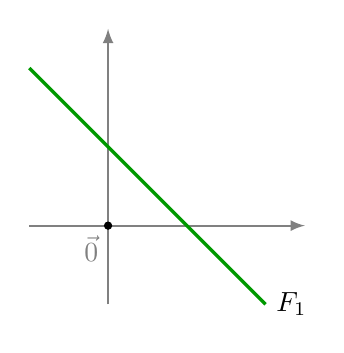
\begin{tikzpicture}

      \draw[->,>=latex,thick, gray] (-1,0)--(2.5,0); % node[below,black] {$x$};
       \draw[->,>=latex,thick, gray] (0,-1)--(0,2.5); % node[right,black] {$y$};
         \fill (0,0) circle (1.5pt);
         \node[below left, gray] at (0,0) {$\vec{0}$};
       \draw[very thick,green!60!black] (-1,2)--(1,0)--+(1,-1)  node[black,right] {$F_1$};


\end{tikzpicture}
\end{Enonce}
\begin{Correction}
Le vecteur nul $(0,0)$ n'appartient pas à $F_1$ donc $F_1$ n'est pas un sous espace vectoriel de $\R^2$.
\end{Correction}
\end{Exemple}
\begin{Exemple}[Fonctions]
\begin{Enonce}Démontrer que les fonctions continues sur $\R$ est un sous-espace vectoriel
  de l'espace vectoriel des fonctions de $\R$ dans $\R$.
\end{Enonce}
\begin{Correction}
La fonction nulle est continue, la somme de deux fonctions continues est continue et une constante fois une fonction continue est une fonction continue.
\end{Correction}
\begin{Enonce}Démontrer que l'ensemble des suites réelles convergentes est un
  sous-espace vectoriel de l'espace vectoriel des suites réelles.
\end{Enonce}
\begin{Correction}
%TODO add reference chapitre suite
La suite nulle est convergente (vers 0), la somme de deux suites convergentes est convergente et une constante fois une suite convergente est une suite convergente.
\end{Correction}
\end{Exemple}

\begin{Exemple}[Matrices]
\begin{Enonce}
Démontrer que l'ensemble des matrices triangulaires supérieures de taille $n$ à coefficients dans $\K$ est un sous-
espace vectoriel de $\MnK$.
\end{Enonce}
\begin{Correction}
La matrice nulle est triangulaire, la somme de deux matrices triangulaires  est une matrice triangulaire et une constante fois une matrice continue est une matrice triangulaire.
\end{Correction}
\end{Exemple}
\subsection{Engendré par une famille}
\begin{Definition}[Sous-espace vectoriel engendré par une famille finie]
Soit  $(\Vect{x}_1,\dots,\Vect{x_p})$ une famille de vecteurs.\\
On appelle l'\defi{espace engendré} l'ensemble des combinaison linéaires de la famille $(\Vect{x}_1,\dots,\Vect{x_p})$, noté \defi{$\VectE  (\mathcal{F})$} :
$$\VectE  (\Vect{x}_1,\dots,\Vect{x_p})=\{ \lambda_1. \Vect{x_1}+\dots + \lambda_p. \Vect{x_p} : \lambda_1,\dots,\lambda_p \in  \K \}.$$
Il s'agit du plus petit sous-espace vectoriel de $E$ contenant la famille $(\Vect{x}_1,\dots,\Vect{x_p})$.\\
Par convention, $\VectE (\emptyset)= \{\Vect{0}_E\}$.\\
\end{Definition}
\begin{Remarque}
 Plus généralement, on peut définir le sous-espace vectoriel engendré
par une famille $(\Vect{x}_i)_{i\in I}$ comme étant l'ensemble des combinaison linéaires de la famille $(\Vect{x}_i)_{i\in I}$.\\
Par exemple,  $\K[X]=\VectE (X^i)_{i\in \N}$.
\end{Remarque}
\begin{Exemple}[Droite vectorielle]
Lorsque que $p=1$ avec $ \Vect{x} \neq \Vect{0}$, $\VectE (\Vect{x}) = \{\lambda .\Vect{x} : \forall \lambda  \in  \K  \}$
est la \defi{droite vectorielle} engendrée par $\Vect{x}$. On la note $\R \Vect{x}$.
\begin{center}
\begin{tikzpicture}[general,scale=1]
         \fill (0,0) circle (1.5pt);
         \node[above left] at (0,0) {$\vec{0_E}$};
\draw [-,color=colordef ] (-1,-0.5) -- (3,1.5)node[right]{$\VectE(\Vect{x}) $};
\draw [->,color=colorprop] (0,0) -- (2,1)node[right]{$\Vect{x}$};
\end{tikzpicture} 
\end{center}
\end{Exemple}
\begin{Exemple}[Plan vectoriel]
Lorsque que $p=2$ avec $ \Vect{x}$ non colinéaire à $\Vect{y}$, $\VectE  (\Vect{x},\Vect{y}) = \{\lambda .\Vect{x}+\mu.\Vect{y} : \forall \lambda ,\mu \in  \K  \}$
est le \defi{plan vectorielle} engendrée par $(\Vect{x},\Vect{y})$. On le note $\R \Vect{x}+\R \Vect{y}$.
\begin{center}
\begin{tikzpicture}[scale=1.3]

        \draw[thick,colordef] (-3,-1)--++(3,-1)--++(2,2)--++(-3,1)--cycle;
        \fill[opacity=0.5,colordef] (-3,-1)--++(3,-1)--++(2,2)--++(-3,1)--cycle;

       \draw[->,>=latex,thick, colorprop] (-0.5,-0.5)--(1,0.1) node[midway, below] {$\Vect{x}$};
       \draw[->,>=latex,thick, colorprop] (-0.5,-0.5)--(-1.3,0.25) node[midway, below left] {$\Vect{y}$};
               \node[above left,colordef] at (2,-2) {$\text{Vect}(\Vect{x},\Vect{y})$};
       \fill (-0.5,-0.5) circle (1.5pt);
         \node[below] at (-0.5,-0.5) {$0$};
\end{tikzpicture}
\end{center}
\end{Exemple}

\subsection{Intersection}
\begin{Proposition}
Soit $F, G$ deux sous espaces vectoriels d'un $\K$-espace vectoriel $E$.\\
Alors l'intersection $F\cap G$ est également un sous espace vectoriel.\\
De même l'intersection $\cap_{i\in I}F_i$
d'une famille quelconque de sous-espaces vectoriels de $E$ est un sous-espace vectoriel.
\end{Proposition}

\begin{Demonstration}
\begin{itemize}
\item \impo{non vide :} comme $F$ et $G$ sont des sous-espaces vectoriels de $E$, $\Vect{0_E}\in F$ et $\Vect{0_E}\in G$ donc $\Vect{0_E}\in F\cap G$
\item \impo{stable par $+$ :} soit $\Vect{x}_1,\Vect{x}_2 \in F\cap G $.\\
Comme $F$ est un sous-espace vectoriel, $\Vect{x}_1+\Vect{x}_2\in F$ car $\Vect{x}_1,\Vect{x}_2 \in F$. De même, $\Vect{x}_1+\Vect{x}_2\in G$. Donc $\Vect{x}_1+\Vect{x}_2\in F\cap G$.
\item
  \impo{stable par $.$ :} soit $\lambda\in \K$ et $\Vect{x}\in F\cap G $.\\
   Comme $F$ est un sous-espace vectoriel,  $\lambda\Vect{x}\in F$. De même,  $\lambda\Vect{x}\in G$. Donc $\lambda\Vect{x}\in F\cap G$.
\end{itemize}
$F\cap G$ est un sous-espace vectoriel de $E$.
\end{Demonstration}


\begin{Exemple}[Intersection de deux plans dans l'espace]
\begin{Enonce}
Démontrer que $D=\{(x,y,z)\in \R^3:  x+3y+z =0\}\cap \{(x,y,z)\in \R^3: z=x\} $ est
 est un sous-espace vectoriel de $\R^3$.
\end{Enonce}
\begin{Correction}
$F=\{(x,y,z)\in \R^3:  x+3y+z =0\}$ et $G=\{(x,y,z)\in \R^3: z=x\}$ sont deux plans vectoriels de $\R^3$. Donc  l'intersection $D=F\cap G$, est un sous espace vectoriel de $\R^3$.
\begin{center}
\begin{tikzpicture}


      \draw[thick,colordef] (-2,0)--++(2,1)--++(3,-1)--++(-2,-1)--cycle;

      \draw[thick,colordef] (-2,0)--++(-2,-1)--++(3,-1)--++(2,1)--cycle;
      \fill[opacity=0.9,colordef] (-2,0)--++(2,1)--++(3,-1)--++(-2,-1)--cycle;

      \draw[thick,colorprop] (-2,0)--++(1,2)--++(3,-1)--++(-1,-2)--cycle;
      \fill[opacity=0.9,colorprop] (-2,0)--++(1,2)--++(3,-1)--++(-1,-2)--cycle;
      \draw[thick,colorprop] (-2,0)--++(-1,-2)--++(3,-1)--++(1,2)--cycle;
      \fill[opacity=0.9,colorprop]  (-2,0)--++(-1,-2)--++(3,-1)--++(1,2)--cycle;

       \fill[opacity=0.9,colordef] (-2,0)--++(-2,-1)--++(3,-1)--++(2,1)--cycle;
     \draw[very thick,green!60!black] (-2,0)--++(3.3,-1.1)-++(-3.6,1.2);
       \node[green!60!black,right] at (1.5,-1.2) {$D$};
       \node[colorprop] at (1.5,1.5) {$F$};
       \node[colordef] at (2.5,-0.5) {$G$};
\end{tikzpicture}
\end{center}

\end{Correction}
\end{Exemple}
\subsection{Somme de sous-espaces vectoriels}

\begin{DefinitionProposition}[Somme]
Soit $E$ un $\K $-espace vectoriel, $F$ et $G$ deux sous-espaces vectoriels de $E$.\\
On appelle \defi{somme} de $F$ et $G$ l'ensemble $ F+G$ des vecteurs de la forme $\Vect{x} +\Vect{y}$
où $\Vect{x}\in F$ et $\Vect{y}\in G$;
autrement dit,
$$  F+G = \{\Vect{x} +\Vect{y} : \Vect{x}\in F,\Vect{y}\in G\}.$$
$F+G$ est un sous espace vectoriel  de $E$.\\
Plus précisément $F+G$ est le plus petit (au sens de l'inclusion) sous espace vectoriel  de $E$ contenant $F$ et $G$.\\

\end{DefinitionProposition}
\begin{Remarque}
Pour construire un sous-espace vectoriel contenant deux sous espaces vectoriels $F$ et $G$, une idée aurait été de considérer l'union $F$ et $G$. Cependant $F\cup G$ n'est presque jamais un sous espace vectoriel.
\begin{center}
\begin{tikzpicture}[general,scale=1]
         \fill (0,0) circle (1.5pt);
         \node[below left, gray] at (0,0) {$\vec{0}$};
\draw [-,color=colordef ] (-1,-0.5) -- (3,1.5)node[right]{$F $};
\draw [->,color=colorprop] (0,0) -- (2,1)node[right]{$\Vect{x}$};
\draw [-,color=colorprop,dashed] (2,1) -- (3,0);
\draw [-,color=colorprop,dashed] (1,-1) -- (3,0);
\draw [-,color=colordef ] (-1,1) -- (2,-2)node[right]{$G $};
\draw [->,color=colorprop] (0,0) -- (1,-1)node[right]{$\Vect{y}$};
\draw [->,color=colorprop] (0,0) -- (3,0)node[right]{$\Vect{x}+\Vect{y}\notin F\cup G$};
\end{tikzpicture} 
\end{center} 
Bien que vecteurs $\Vect{x},\Vect{y}\in F\cup G$, leur somme   $\Vect{x}+\Vect{y}$ n'appartient pas à $ F \cup G.$ 
\end{Remarque}


\begin{Demonstration}
\begin{itemize}
\item \impo{non vide :}
$\Vect{0}\in F$ et $G$ d'où $\Vect{0}=\underbrace{\Vect{0}}_{\in F}+\underbrace{\Vect{0}}_{\in G}\in F+G.$
\item \impo{stable par $+$ :}
Soit $\Vect{x_1}+\Vect{y_1},\Vect{x_2}+\Vect{y_2} \in  F+G.$\\
$\Vect{x_1}+\Vect{y_1}+\Vect{x_2}+\Vect{y_2} =\underbrace{\Vect{x_1}+\Vect{x_2}}_{\in F}+\underbrace{\Vect{y_1}+\Vect{y_2}}_{\in G}\in  F+G.$
\item
  \impo{stable par $.$ :}
Soit $\lambda\in \R$ et $\Vect{x}+\Vect{y}  \in  F+G.$\\
$\lambda (\Vect{x}+\Vect{y})=\underbrace{\lambda\Vect{x}}_{\in F}+\underbrace{\lambda\Vect{y}}_{\in G} \in  F+G.$
\end{itemize}
\end{Demonstration}
\begin{Exemple}[Somme de deux droites vectorielles]
Soit $F$ et $G$ deux droite vectorielles distinctes. La somme $F+G$ est un plan vectoriel.
\begin{center}
\begin{tikzpicture}[general,scale=1]
\draw [color=colordef,fill=colordef] (-1.5,-2) -- (-3.5,-1.5) -- (1.5,2) -- (3.5,1.5)node[right]{$F+G$}; -- cycle ;
\draw [very thick,color=colorprop] (-1.6,-2) -- (1.6,2)node[above right]{$F$};
\draw [very thick,color=colorprop] (-2.2,-0.6) -- (2.2,0.6)node[right]{$G$};
        \fill (0,0) circle (1.5pt);
         \node[below left, gray] at (0,0) {$\vec{0}$};
\end{tikzpicture} 

\end{center}
\end{Exemple}
\subsection{Somme directe de sous espaces vectoriels}
\begin{Definition}[Somme directe]
On dit que la somme $F+G$ est \defi{directe} si tout vecteur de la somme se décompose \defi{de façon unique} sous la forme $\Vect{x} +\Vect{y}$ où $\Vect{x}\in F$ et $\Vect{y}\in G$, ce qui revient à dire :
$$ \forall \Vect{x} , \Vect{x}'\in F,\forall \Vect{y} , \Vect{y}'\in G: \Vect{x} + \Vect{y} = \Vect{x}' + \Vect{y}'\Rightarrow  \Vect{x} = \Vect{x}'\text{ et }  \Vect{y} = \Vect{y}'.$$
On note alors la somme $F\oplus G$ la somme $F + G$ pour indiquer qu'il y a somme directe.\\
De même, la somme $F_1\oplus F_2\oplus\dots\oplus F_p$ est \defi{directe} si tout vecteur de la somme se décompose \defi{de façon unique} sous la forme $\Vect{x_1} +\Vect{x_2}+ \dots + \Vect{x_p}$ où $\Vect{x_1}\in F_1$, ..., ,$\Vect{x_p}\in F_p$.
\end{Definition}
\begin{Proposition}[Caractérisation de la somme directe]
La somme $F+G$ est directe si et seulement si
$$ \forall \Vect{x} \in F, \forall \Vect{y} \in G:\quad 
  \Vect{x} +\Vect{y} = \Vect{0_E} \Rightarrow \Vect{x} =  \Vect{y} = \Vect{0_E}.$$
De même  la somme $F_1+\dots+F_p$ est directe si et seulement si
$$\Vect{x_1}\in F_1,  ..., \Vect{x_p}\in F_p:\quad
 \Vect{x_1} + \dots + \Vect{x_p} = \Vect{0_E} \Rightarrow \Vect{x_1} =\dots=\Vect{x_p}= \Vect{0_E}.$$
\end{Proposition}
\begin{Demonstration}
\begin{itemize}
\item \impo{$(\Longrightarrow)$} :
Soit $\Vect{x} \in F$ et $\Vect{y} \in G$ tel que $\Vect{x} + \Vect{y}=\Vect{0}$. On a aussi $\underbrace{\Vect{0}}_{\in F}+\underbrace{\Vect{0}}_{\in G}=\Vect{0}.$ L'unicité de décomposition permet d'identifier  $\Vect{x}=\Vect{0}$ et $\Vect{y}=\Vect{0}$.
\item \impo{$(\Longleftarrow)$} :
Supposons qu'un vecteur $\Vect{z} \in F+G$  se décompose de 2 façons :$\Vect{z}= \underbrace{\Vect{x}}_{\in F} + \underbrace{\Vect{y}}_{\in G}$ et $\Vect{z}= \underbrace{\Vect{x'}}_{\in F} + \underbrace{\Vect{y}}_{\in G}$. \\
On soustrait ces deux égalités :
$$\Vect{0}= \underbrace{\Vect{x} -\Vect{x'} }_{\in F}+\underbrace{\Vect{y} -\Vect{y'} }_{\in G}.$$
D'après l'hypothèse, on a   $\Vect{x} -\Vect{x'}=\Vect{0}$ et $\Vect{y} -\Vect{y'}=\Vect{0}$, d'où $\Vect{x} =\Vect{x'}$ et $\Vect{y}=\Vect{y'}.$ 
\end{itemize}
\end{Demonstration}
\begin{Proposition}[Caractérisation de la somme directe]
La somme $F+G$ est directe si et seulement si $F\cap G = \{\Vect{0_E}\}$.
\end{Proposition}
\begin{Remarque}
Cette caractérisation ne se généralise pas (simplement) pour $p > 2$.\\
Contre-exemple, soit $\Vect{x_1} = (1,0)$, $\Vect{x_2} = (0,1)$ et $\Vect{x_3} = (1,1)$ trois vecteurs de $\R^2$.\\
Bien que $\R \Vect{x_1} \cap \R \Vect{x_2} = \R \Vect{x_1} \cap \R \Vect{x_3} = \R \Vect{x_2} \cap \R \Vect{x_3} = \{(0,0)\}$,
La somme $\R \Vect{x_1} + \R \Vect{x_2} + \R \Vect{x_3}$ n'est pas directe.\\
En effet, le vecteur $(1,1)$ se décompose de deux manière  $$(1,1)=\overbrace{0(1,0)}^{\in \R \Vect{x_1} }+\overbrace{0(0,1)}^{\in \R \Vect{x_2} }+ \overbrace{1(1,1)}^{\in \R \Vect{x_3}}\text{ et }(1,1)=\overbrace{1(1,0)}^{\in \R \Vect{x_1} }+\overbrace{1(0,1)}^{\in \R \Vect{x_2} }+ \overbrace{0(1,1)}^{\in \R \Vect{x_3}}.$$
\end{Remarque}
\begin{Demonstration}
\begin{itemize}
\item \impo{$(\Longrightarrow)$ :}  
\begin{itemize}
\item \impo{$\{\Vect{0_E}\}   \subset  F\cap G$} :
$\Vect{0_E}\in F,G$ donc $\Vect{0_E}\in F\cap G .$ 
\item \impo{$F\cap G  \subset \{\Vect{0_E}\} $} :
Soit $\Vect{x}\in F\cap G$. 
On a $\Vect{0}= \underbrace{\Vect{x}}_{\in F} + \underbrace{-\Vect{x}}_{\in G}= \underbrace{\Vect{0}}_{\in F} + \underbrace{\Vect{0}}_{\in G}$. Par unicité de la décomposition, on identifie $\Vect{x}=\Vect{0}.$
\end{itemize}
Du fait de la double inclusion, on a $F\cap G = \{\Vect{0_E}\}.$
\item \textit{$(\Longleftarrow)$ :}\\
Supposons qu'un $\Vect{z} \in F+G$  se décompose de 2 façons :$\Vect{z}= \underbrace{\Vect{x}}_{\in F} + \underbrace{\Vect{y}}_{\in G}$ et $\Vect{z}= \underbrace{\Vect{x'}}_{\in F} + \underbrace{\Vect{y}}_{\in G}$. \\
On soustrait ces deux égalités :
$$\underbrace{\Vect{x} -\Vect{x'} }_{\in F}=\underbrace{\Vect{y'} -\Vect{y} }_{\in G}.$$
Comme $F\cap G = \{\Vect{0_E}\}$, on a $\Vect{x} -\Vect{x'}=\Vect{0}$ et $\Vect{y} -\Vect{y'} =\Vect{0}$, d'où l'unicité de la décomposition avec $\Vect{x} =\Vect{x'}$ et $\Vect{x}=\Vect{y'}.$
\end{itemize}
\end{Demonstration}
\begin{Remarque}
Pour démontrer que $F\cap G = \{\Vect{0_E}\}$, dans le raisonnement de la double inclusion, on omettra l'inclusion $F\cap G = \{\Vect{0_E}\}$ qui est évidente. En effet $\Vect{0_E}\in F,G$ car $F$ et $G$ sont des sous espaces vectoriels de $E$. 
\end{Remarque}

\begin{Exemple} Géométriquement, l'intersection entre deux plans vectoriels distincts, $F$ et $G$, est une droite vectoriel, donc la somme n'est pas directe.
\begin{center}
\begin{tikzpicture}


      \draw[thick,colordef] (-2,0)--++(2,1)--++(3,-1)--++(-2,-1)--cycle;

      \draw[thick,colordef] (-2,0)--++(-2,-1)--++(3,-1)--++(2,1)--cycle;
      \fill[opacity=0.9,colordef] (-2,0)--++(2,1)--++(3,-1)--++(-2,-1)--cycle;

      \draw[thick,colorprop] (-2,0)--++(1,2)--++(3,-1)--++(-1,-2)--cycle;
      \fill[opacity=0.9,colorprop] (-2,0)--++(1,2)--++(3,-1)--++(-1,-2)--cycle;
      \draw[thick,colorprop] (-2,0)--++(-1,-2)--++(3,-1)--++(1,2)--cycle;
      \fill[opacity=0.9,colorprop]  (-2,0)--++(-1,-2)--++(3,-1)--++(1,2)--cycle;

       \fill[opacity=0.9,colordef] (-2,0)--++(-2,-1)--++(3,-1)--++(2,1)--cycle;
     \draw[very thick,green!60!black] (-2,0)--++(3.3,-1.1)-++(-3.6,1.2);
       \node[green!60!black,right] at (1.5,-1.2) {$F\cap G$};
       \node[colorprop] at (1.5,1.5) {$F$};
       \node[colordef] at (2.5,-0.5) {$G$};
\end{tikzpicture}
\end{center}
\begin{Enonce}
Démontrer que  $F=\{(x,y,z)\in\R^3: x+y+z=0\}$ et $G=\{(x,y,z)\in\R^3: x-y+z=0\}$ ne sont pas en somme directe.
\end{Enonce}
\begin{Correction}
 On a :
$$\begin{aligned}
 (x,y,z)\in F \cap G & \Leftrightarrow \begin{cases}x+y+z=0 \\ x-y+z=0 \end{cases}\\
 & \Leftrightarrow \begin{cases}x+y+z=0 \\ -2y=0 \quad L_2\leftarrow L_2 - L_1\end{cases}\\
 & \Leftrightarrow \begin{cases}x+z=0 \\ y=0 \end{cases}\\
 & \Leftrightarrow  z=z, x=-z , y=0 \\
 & \Leftrightarrow  (x,y,z) = z(-1,0,1)
 \end{aligned}$$
Finalement  $F \cap G = \VectE ( -1,0,1)$ et $F$ et $G$ ne sont pas en somme directe. 
\end{Correction}
\end{Exemple}
\subsection{Sous-espaces vectoriels supplémentaires}
\begin{Definition}[Sous-espaces vectoriels supplémentaires]
Si la somme $F+G$ est directe et égale à $E$,
on dit que $F$ et $G$ sont \defi{supplémentaires}, et on note
$$ E = F\oplus G.$$
C'est-à-dire que tout vecteur de $E$ se décompose d'une unique manière de la somme d'un élément de $F$ et d'un élément de $G$ :
$$\forall \vec{x} \in E,\quad \exists !  (\vec{y}, \vec{z}) \in F \times G:\quad  \vec{x} = \vec{y} + \vec{z}.$$
De même si la somme $F_1+F_1+\dots+F_P$ est directe et égale à $E$, on dit que $F_1,F_2,\dots,F_p$ sont \defi{supplémentaires}.
\begin{center}
\begin{tikzpicture}
        \draw[thick,colorprop] (-4,-1)--++(4,-1)--++(2,2)--++(-4,1)--cycle;
        \fill[opacity=0.5,colorprop] (-4,-1)--++(4,-1)--++(2,2)--++(-4,1)--cycle;

      \node[colorprop,above left] at (1.5,0.3) {$F$};

      \draw[colorprop,  thick] (-1,-0.5)--++(0.5,2) node[above] {$G$};
      \draw[colorprop,  thick, dotted] (-1,-0.5)--++(-0.3,-1.20);
      \draw[colorprop,  thick] (-1.3,-1.7)--++(-0.1,-0.4);

	\draw[colordef,dashed] (-0.65,0.9)--++(1,0.25);	
	\draw[colordef,dashed] (0,-0.25)--++(0.35,1.4);	
	\draw[->,colordef] (-1,-0.5)--++(0.35,1.4)node[left] {$\vec{z}$};
	\draw[->,colordef] (-1,-0.5)--++(1,0.25)node[right] {$\vec{y}$};
	\draw[->,colordef] (-1,-0.5)--++(1.35,1.65)node[above] {$\vec{x}=\vec{y}+\vec{z}$};
         \fill (-1,-0.5) circle (1.5pt);
         \node[above left] at (-1,-0.5) {$\Vec{0_E}$};
         
         \draw[thick,colorprop] (-4,-1)--++(4,-1)--++(2,2)--++(-4,1)--cycle;
\end{tikzpicture}
\end{center}
\end{Definition}
\begin{Remarque}
Il n'y a pas unicité du supplémentaire. Donc il est interdit d'écrire "du supplémentaire d'un sous espace vectoriel".\\
Il ne faut pas confondre "supplémentaire" et "complémentaire". 
\end{Remarque}
\begin{Exemple}[Espace]
\begin{Enonce}
Démontrer que les sous-espaces vectoriels $F$ et $G$ de $\R^3$ définis par
$$F=\big\{ (x,y,z) \in \R^3\mid x-y-z=0\big\} \qquad \text { et } \qquad
G=\big\{(x,y,z) \in \R^3 \mid y=z=0\big\}$$
sont supplémentaires dans $\R^3$.
\end{Enonce}
\begin{Correction}
Soit $(x,y,z)\in\R^3$.
\begin{itemize}
 \item \impo{Analyse} :  Supposons qu'il existe $(x_1,y_1,z_1)\in F$ et $(x_2,y_2,z_2)\in G$ tel que 
  $(x,y,z) =(x_1,y_1,z_1)+(x_2,y_2,z_2)$.\\
  Comme $(x_1,y_1,z_1)\in F$, $(x_1,y_1,z_1)=(\overbrace{y_1+z_1}^{x_1-y_1-z_1=0}, y_1,z_1)$ et comme $(x_2,y_2,z_2)\in G$, $(x_2,y_2,z_2)=(x_2, 0,0)$.\\
  Ainsi
  $$(x,y,z) =(x_1,y_1,z_1)+(x_2,y_2,z_2)=(y_1+z_1+x_2,y_1,z_1).$$
  On obtient $y_1=y$, $z_1=z$, $x_2=x-y-z$. D'où l'unicité de la décomposition.
  \item \impo{Synthèse} : On vérifie que $(x,y,z)=\overbrace{(y+z,y,z)}^{\in F}+ \overbrace{(x-y-z, 0,0)}^{\in G}$. D'où l'existence de la décomposition.
\end{itemize}
$F \oplus G=\R^3$.
\end{Correction}
\end{Exemple}


\begin{Exemple}[Polynôme]
\begin{Enonce}
Soit $P \in \K[X]$ non nul de degré $n$.\\
Démontrer que $ \K[X] = P \K[X] \oplus \K_{n-1}[X]$ où : $P\K[X] =\{ PQ | Q \in \K[X]\}$.
\end{Enonce}
\begin{Correction}
Soit $A\in \K[X]$.
D'après le théorème de la division euclidienne, 
$$\exists ! (Q,R) \in \K[X] \times \K_{n-1}[X]:\quad A = \overbrace{PQ}^{\in P\K[X]}+ \overbrace{R}^{\in \K_{n-1}[X]}.$$
Donc $ \K[X] = P \K[X] \oplus \K_{n-1}[X]$.
\end{Correction}
\end{Exemple}


\begin{Exemple}[Fonctions pairs et impairs]
\begin{Enonce}
Soit $\R$-espace vectoriel $\SpaceFonction{\R}{\R}$
des fonctions de $\R$ dans $\R$.\\
Démontrer que le sous-espace
vectoriel des fonctions paires $\mathcal{P}$ et le sous-espace
vectoriel des fonctions impaires $\mathcal{I}$ sont supplémentaires.
\end{Enonce}
\begin{Correction}
Soit $f\in \SpaceFonction{\R}{\R}$.
\begin{itemize}
 \item \impo{Analyse} : Supposons qu'il existe  $g\in\mathcal{P}$ et $h\in\mathcal{I}$ tel que $f=g+h$.\\
  Soit $x\in\R$.\\	
  D'une part, $f(x)=g(x)+h(x)$, et d'autre part, $f(-x)=g(-x)+h(-x)=g(x)-h(x)$.\\
  Par somme et différence, obtient
  $$g(x)=\frac{f(x)+f(-x)}2 \qquad \text{ et } \qquad h(x)=\frac{f(x)-f(-x)}2.$$
	D'où l'unicité de la décomposition.	\\
  \impo{Synthèse.} Soit $x\in\R$.\\ 
  On pose $g,h$ définit par $$\forall x\in\R:\quad g(x)=\frac{f(x)+f(-x)}2 \text{ et }h(x)=\frac{f(x)-f(-x)}2.
  $$
  On a $f=g+h$ et d'autre part $g \in \mathcal{P}$ car 
  $$\forall x\in\R: g(-x)=\frac{f(-x)+f(-(-x))}2=\frac{f(x)+f(-x)}2=g(x)$$ et $h\in\mathcal{I}$ car $$\forall x\in\R: h(-x)=-h(x).$$ D'où l'existence de la décomposition.	
\end{itemize}
$\mathcal{P}\oplus\mathcal{I}=\mathcal{F}(\R , \R)$.
\end{Correction}
\end{Exemple}

\begin{Proposition}[Existence d'un supplémentaire]
Dans un espace vectoriel de dimension finie, tout sous espace vectoriel admet un supplémentaire.\\
Autrement dit, soit $E$ est un espace vectoriel de dimension finie et $F$ un sous espace vectoriel de $E$.\\
Alors il existe un sous espace vectoriel $G$ de $E$ tel que $E = F \oplus G$.
\end{Proposition}
\begin{Demonstration}
La démonstration fait appel à des résultats ultérieurs (à but pédagogique, cette proposition est ici).\\
Soit $\mathcal{B}_1$ une base de $F$ que l'on complète avec $\mathcal{B}_2$ pour former une base de $E$.\\
Si on pose $G$ l'espace vectoriel engendrée par  $\mathcal{B}_2$, alors $E = F \oplus G$.  
\end{Demonstration}
%\begin{Enonce}
%Démontrer que $\R_{n-1}[X]$ et $\VectE (X^n)$ sont supplémentaires dans $\R_n[X]$
%\end{Enonce}
%
%\begin{Correction}
%\begin{itemize}
%\item \impo{$\R_n[X]=\R_{n-1}[X]+ \VectE (X^n) $} :\\
%Soit $P =a_0+a_1 X+\dots+a_{n-1} X^{n-1}+a_{n} X^{n}\in \R_n[X].$
%On a $$P =\overbrace{a_0+a_1 X+\dots+a_{n-1} X^{n-1}}^{\in \R_{n-1}[X]}+\overbrace{a_{n} X^{n}}^{\in \VectE (X^n)}.$$
%\item \impo{$\R_{n-1}[X]\cap  \VectE (X^n)=\{\Vect{0}_{\R_n[X]}\}$ :}\\
%Soit $P \in \R_{n-1}[X]\cap \VectE (X^n)$.\\
%Comme $P \in \R_{n-1}[X]$, on a $deg(P)<n$. Comme  $P \in \VectE (X^n)$, on a $P=\lambda X^n$. Si $\lambda\neq 0$, on a $deg(P=\lambda X^n)=n$, ce qui impossible car $deg(P)<n$.\\
%Ainsi  $\lambda= 0$et donc  $P=0$.  
%\end{itemize}
%\end{Correction}
%\end{Exemple}
% -----------------------------------------------------------------------------
\section{Base}

\subsection{Famille génératrice}
\begin{Definition}[Famille génératrice]
Une famille finie  $(\Vect{x}_1,\dots,\Vect{x_p})$ est \defi{génératrice} de $E$ si tout vecteur de $E$ est combinaison linéaire de  $(\Vect{x}_1,\dots,\Vect{x_p})$, c'est à dire si $\VectE (\Vect{x}_1,\dots,\Vect{x_p}) = E$, c'est à dire si 
$$ \forall \Vect{x} \in E,\exists \lambda_1,\dots,\lambda_p \in \K,\quad \Vect{x} = \lambda_1 \Vect{x_1}+ \lambda_2 \Vect{x_2}+\dots +\lambda_p \Vect{x_p}.$$
\end{Definition}
\begin{Texte}
Une famille génératrice garantit \defi{l'existence pour tout vecteur d'une décomposition comme combinaison linéaire.}
\end{Texte}
\begin{Exemple}[Plan]
\begin{Enonce}
Démontrer que la famille  $\{(1,1), (0,1), (1,-1)\}$  est génératrice de $\R^2$.
\end{Enonce}
\begin{Correction}
Soit $(x,y)\in\R^2$, on a :
$$(x,y)=\frac{x+y}{2}(1,1)+ \frac{x-y}{2} (1,-1).$$
En revanche,  la combinaison linéaire n'est pas unique car on a aussi $(x,y)= x(1,1)+(y-1)(0,1).$
\end{Correction}
\end{Exemple}
\begin{Exemple}[Espace]
\begin{Enonce}
Déterminer une famille génératrice de l'espace vectoriel $E =\{ (x, y, z) \in \R | x + 2y - z = 0 \}$
\end{Enonce}
\begin{Correction}
Soit $(x, y, y) \in \R^3$.
$$ (x, y, z) \in E \Longleftrightarrow z = x + 2y.$$
Donc $E =\{ (x, y, x + 2y)  | x, y \in \R\}=\{ x(1, 0, 1)+y(0,1,1)  | x, y \in \R\} = \VectE 
(1, 0, 1),(0, 1, 2)$.
\end{Correction}
\end{Exemple}

\begin{Exemple}[Espace]
\begin{Enonce}
Démontrer que la famille $(\left(\begin{smallmatrix}1\\1\\1\end{smallmatrix}\right),\left(\begin{smallmatrix}1\\2\\3\end{smallmatrix}\right)$ n'est pas génératrice de $\R^3$.
\end{Enonce}
\begin{Correction}
\impo{Contre-exemple} soit $\left(\begin{smallmatrix}0\\1\\0\end{smallmatrix}\right)\in\R^3$. Si ce vecteur est combinaison linéaire de la famille, il existe $\lambda_1,\lambda_2 \in \R$ tel que
$\left(\begin{smallmatrix}0\\1\\0\end{smallmatrix}\right)=\lambda_1 (\left(\begin{smallmatrix}1\\1\\1\end{smallmatrix}\right)+\left(\begin{smallmatrix}1\\2\\3\end{smallmatrix}\right)$.
D'où le système linéaire :
$$
\left\{\begin{array}{rcl}
\lambda_1 + \lambda_2 & = & 0\\
\lambda_1 + 2\lambda_2 & = & 1\\
\lambda_1 + 3\lambda_2 & = & 0
\end{array}\right.
$$
En soustrayant la seconde ligne à la première, on obtient $\lambda_2=0$, puis $\lambda_1=0$.  D'où $\left(\begin{smallmatrix}0\\1\\0\end{smallmatrix}\right)= 0$ ce qui est impossible. Donc la famille $(\left(\begin{smallmatrix}1\\1\\1\end{smallmatrix}\right),\left(\begin{smallmatrix}1\\2\\3\end{smallmatrix}\right))$ n'est pas génératrice de $\R^3$. 
\end{Correction}
\end{Exemple}

\subsection{Famille libre }
\begin{Definition}[Famille libre]
Une famille  $(\Vect{x}_1,\dots,\Vect{x_p})$ est \defi{libre} si tout vecteur s'exprime de manière unique comme combinaison linéaire de la famille, c'est à dire si 
$$ \forall \lambda_1,\dots,\lambda_p,\beta_1,\dots,\beta_p \in \K,\quad \left(\lambda_1 \Vect{x_1}+ \dots +\lambda_p \Vect{x_p}=\beta_1 \Vect{x_1}+ \dots +\beta_p \Vect{x_p}\Longrightarrow  \lambda_1=\beta_1,\dots,\lambda_p=\beta_p\right)  .$$
Dans le cas contraire, on dit que la famille est \defi{liée} ou \defi{linéairement dépendante}.
\end{Definition}
\begin{Texte}
Une famille libre garantit \defi{l'unicité des coefficients dans les combinaisons linéaires,
donc le possibilité de pratiquer des identifications.}\\
Par exemple, si on a $\sum_{i=0}^n a_i (X+1)^i=\sum_{i=0}^n i (X+1)^i$, alors $a_i=i\; \forall i\in\Intf{0}{n}$ car la famille $((X+1)^i)_{0\leq i\leq n }$ est libre. 
\end{Texte}
\begin{Remarque}
La famille vide $\varnothing$ est libre.
\end{Remarque}
\begin{Exemple}
\begin{Enonce}
Démontrer que la famille  $\{(1,1), (0,1), (1,-1)\}$  n'est pas libre dans $\R^2$.
\end{Enonce}
\begin{Correction}
Comme  $(1,1)-2(0,1)+0(1,-1)=1(1,-1)+0(0,1)+0(1,-1)$, un même vecteur s'exprime de deux manières distinctes comme combinaison linéaire de la famille. Donc la famille n'est pas libre.
\end{Correction}
\end{Exemple}


\begin{Proposition}[Caractérisation d'une famille libre]
Une famille  $(\Vect{x_1},\dots,\Vect{x_p})$ est \propri{libre} si et seulement si 
$$ \forall \lambda_1,\dots,\lambda_p   \in \K,\quad  \lambda _1 \Vect{x_1}+\dots+\lambda_p \Vect{x_p} = \Vect{0_E} \Rightarrow \lambda _1=\lambda _2=\dots=\lambda_p= 0  .$$
\end{Proposition}
\begin{Demonstration}
\begin{itemize}
\item \impo{$(\Longrightarrow)$} :
Soit $\lambda_1,\dots,\lambda_p   \in \K$ tel que$\lambda _1 \Vect{x_1}+\dots+\lambda _n \Vect{x_n} = \Vect{0_E}$. Comme $\Vect{0_E}=0 \Vect{x_1}+\dots+0 \Vect{x_n} $. Par identification, on obtient $\lambda _1=\dots=\lambda_p= 0$.
\item \impo{$(\Longleftarrow)$} :
Soit $\lambda_1,\dots,\lambda_p,\beta_1,\dots,\beta_p \in \K$ tel que $ \lambda_1 \Vect{x_1}+ \dots +\lambda_p \Vect{x_p}=\beta_1 \Vect{x_1}+ \dots +\beta_p \Vect{x_p}.$\\
Par soustraction, on obtient :
$$ (\lambda_1-\beta_1) \Vect{x_1}+ \dots +(\lambda_p-\beta_p) \Vect{x_p}=\Vect{0_E} .$$
D'après l'hypothèse,  $\lambda_1-\beta_1=0,\dots,\lambda_p-\beta_p=0$, donc $\lambda_1=\beta_1,\dots,\lambda_p=\beta_p.$
\end{itemize}
\end{Demonstration}
\begin{Proposition}[Caractérisation d'une famille liée]
Une famille  $(\Vect{x_1},\dots,\Vect{x_p})$ est \propri{liée} si et seulement si au moins un des vecteurs de la famille est combinaison linéaire des autres vecteurs de la famille.
\end{Proposition}
\begin{Demonstration}
\begin{itemize}
\item \impo{$(\Rightarrow)$} : Supposons que la famille est liée. D'après la caractérisation d'une famille libre, il existe  une relation 
$$\lambda _1 \Vect{x_1}+\dots+\lambda _n \Vect{x_p} = \Vect{0_E}$$
avec un $\lambda_k\neq 0$ pour au moins un $k\in\Intf{1}{p}$. Par soustraction de tous les autres termes, on obtient
$$\lambda_k \Vect{x_ k}=-\lambda_1\Vect{x_1}-\cdots-\lambda_{k-1}\Vect{x_{k-1}}-\lambda_{k+1}\Vect{x_{k+1}}-\cdots-\lambda_p \Vect{x_p}.$$ 
Comme $\lambda_k\neq 0$, on peut diviser cette égalité par $\lambda_k$ et l'on obtient :
$$ \Vect{x_ k}=-\frac{\lambda_1}{\lambda_k}\Vect{x_1}-\cdots-\frac{\lambda_{k-1}}{\lambda_k}\Vect{x_{k-1}}-\frac{\lambda_{k+1}}{\lambda_k}\Vect{x_{k+1}}-\cdots-\frac{\lambda_p}{\lambda_k} \Vect{x_p}.$$ 
Donc $\Vect{x_ k}$ est combinaison linéaire des autres vecteurs.
\item \impo{$(\Leftarrow)$} : Supposons qu'il existe $k\in\Intf{1}{p}$ tel que 
$$\Vect{x_ k}=\lambda_1\Vect{x_1}+\cdots+\lambda_{k-1}\Vect{x_{k-1}}+\lambda_{k+1}\Vect{x_{k+1}}+\cdots+\lambda_p \Vect{x_p}.$$ 
Par soustraction, on obtient :
$$\lambda_1\Vect{x_1}+\cdots+\lambda_{k-1}\Vect{x_{k-1}}+\Vect{x_ k}+\lambda_{k+1}\Vect{x_{k+1}}+\cdots+\lambda_p \Vect{x_p}= \Vect{0_E}.$$ 
Comme $1\neq 0$, la famille est liée d'après la caractérisation d'une famille libre.
\end{itemize}
\end{Demonstration}

\begin{Remarque}[Interprétation Géométrique]
\begin{itemize}
\item Dans $\R^2$ ou $\R^3$, deux vecteurs sont linéairement dépendants si et seulement s'ils sont colinéaires.
Ils sont donc sur une même droite vectorielle.
\begin{center}
\begin{tikzpicture}
       \draw[gray] (-5,-1.66)--(5,1.66) ;
       \draw[->,>=latex,thick, colordef] (0,0)--(3,1) node[midway, below right] {$\Vect{x_1}$};
       \draw[->,>=latex,thick, colordef] (0,0)--(-3/2,-1/2) node[midway, below right] {$\Vect{x_2}$};
               \fill (0,0) circle (1.5pt);
         \node[ left, gray] at (0,0) {$\vec{0}$};
\end{tikzpicture}
\end{center}
\item Dans $\R^3$, trois vecteurs sont linéairement dépendants si et seulement s'ils sont coplanaires.
Ils sont donc dans un même plan vectoriel.
\begin{center}
\begin{tikzpicture}
     \fill[colorprop, opacity=0.5] (0,0)--(.5,1)--(3.5, 1.5)--(3,0.5);
      \draw[->,>=latex,thick,gray] (0,0)--(2,0) node[below,black] {$y$};
      \draw[->,>=latex,thick,gray] (0,0)--(0,2) node[right,black] {$z$};
       \draw[->,>=latex,thick,gray] (0,0)--(-1,-1.25) node[left,black] {$x$};

  \draw[->,>=latex,thick, colordef] (0,0)--(3,0.5) node[below right] {$\Vect{x_1}$};
  \draw[->,>=latex,thick, colordef] (0,0)--(.5,1) node[above] {$\Vect{x_2}$};
 \draw[->,>=latex,thick, colordef] (0,0)--(3.5,1.5) node[above] {$\Vect{x_3}$};
   \draw[dashed,colordef] (0.5,1)--(3.5,1.5)--(3,0.5);
        \fill (0,0) circle (1.5pt);
         \node[ left, gray] at (0,0) {$\vec{0}$};
\end{tikzpicture}
\end{center}
\end{itemize}
\end{Remarque}
\begin{Exemple}[Espace]
\begin{Enonce} 
Démontrer que la famille 
$\left(\begin{pmatrix}1\\2\\3\end{pmatrix},\begin{pmatrix}4\\5\\6\end{pmatrix},\begin{pmatrix}2\\1\\0\end{pmatrix}\right)$ 
n'est pas libre.
\end{Enonce}
\begin{Correction}
Soit $\lambda_1, \lambda_2, \lambda_{3}\in\K$ tel que
$$\lambda_1\left(\begin{smallmatrix}
1\\2\\3
\end{smallmatrix}\right)
+\lambda_2\left(\begin{smallmatrix}
4\\5\\6
\end{smallmatrix}\right)
+\lambda_3\left(\begin{smallmatrix}
2\\1\\0
\end{smallmatrix}\right) =
\left(\begin{smallmatrix}
0\\0\\0
\end{smallmatrix}\right)$$
ce qui équivaut au système :


$$\begin{aligned}
&\left \{\begin{matrix}
\lambda_1&+&4\lambda_2&+&2 \lambda_{3}&=&0 \\
2\lambda_1&+&5\lambda_2&+&\lambda_{3}&=&0\\
3\lambda_1&+&6\lambda_2&&&=&0\\
\end{matrix}\right.\\
\Leftrightarrow&
\left \{\begin{matrix}
\lambda_1&+&4\lambda_2&+&2 \lambda_{3}&=&0& \\
&-&3\lambda_2&-&3\lambda_{3}&=&0 &\quad L_2\leftarrow L_2-2L_1\\
&-&6\lambda_2&-&6\lambda_{3}&=&0&\quad L_3\leftarrow L_3-3L_1\\
\end{matrix}\right.\\
\Leftrightarrow& \left \{\begin{matrix}
\lambda_1&+&4\lambda_2&+&2 \lambda_{3}&=&0& \\
&&\lambda_2&+&\lambda_{3}&=&0 &\quad L_2\leftarrow \frac{1}{3}L_2\\
&&&&&& &\quad \text{Supprimer car }L_3=L_2
\end{matrix}\right.\\
\Leftrightarrow&
\left \{ \begin{matrix}
\lambda_1&& &-&2 \lambda_{3}&=&0 \\ L_1 \leftarrow L_1 - 4L_2 
&&\lambda_2&+&\lambda_{3}&=&0\\
\end{matrix}\right .
\end{aligned}
$$
Ce système a une infinité de solutions et en prenant par exemple $\lambda_3=1$
on obtient $\lambda_1=2$ et $\lambda_2=-1$. On vérifie que
$$2\begin{pmatrix}
1\\2\\3
\end{pmatrix} -\begin{pmatrix}
4\\5\\6
\end{pmatrix} +\begin{pmatrix}
2\\1\\0
\end{pmatrix}=
\begin{pmatrix}0\cr 0\cr 0\cr \end{pmatrix}.$$
La famille
$\left(\begin{pmatrix}
1\\2\\3
\end{pmatrix},
\begin{pmatrix}
4\\5\\6
\end{pmatrix},
\begin{pmatrix}
2\\1\\0
\end{pmatrix}\right)$ est donc une famille liée.
\end{Correction}
\end{Exemple}
\begin{Exemple}[Polynôme]
\begin{Enonce}
Démontrer que la famille $( (1-X),(5+3X-2X^2),(1+3X-X^2))$ est liée.
\end{Enonce}
\begin{Correction}
On  a $3(1-X) - (5+3X-2X^2) + 2(1+3X-X^2) = 0.$ donc la famille est liée.
\end{Correction}
\end{Exemple}


\begin{Exemple}[Exemple]
\begin{Enonce}
Démontrer que la famille  $(\cos, \sin)$ est libre dans le $\R$-espace vectoriel $\SpaceFonction{\R}{\R}$.
\end{Enonce}
\begin{Correction} 
Soit $\lambda,\mu\in\K$ tel que $\lambda \cos+\mu \sin =0$. Cela équivaut à
$$\forall x \in \R: \qquad \lambda \cos(x) + \mu \sin(x)=0.  $$
En particulier, pour $x=0$, cette égalité donne $\lambda =0$. Et pour
$x=\frac{\pi}2$, elle donne $\mu=0$.\\
Donc la famille
$(\cos , \sin)$ est libre.
\end{Correction}
\end{Exemple}

\subsection{Base}
\begin{Definition}[Base]
On dit que la famille $\mathcal{B}=(\Vect{e}_1,\dots,\Vect{e_p})$ est une \defi{base} de $E$ si elle est libre et génératrice, c'est-à-dire si tout vecteur de
$E$ s'exprime de manière unique comme combinaison linéaire de $\mathcal{B}$, c'est-à-dire,
$$ \forall \Vect{x}\in E, \exists !  \lambda_1,\dots,\lambda_p   \in \K ,\quad  \Vect{x} = \lambda_1 \Vect{e_1}+ \lambda_2 \Vect{e_2}+\dots +\lambda_p \Vect{e_p}.$$
 $(\lambda_1, \dots , \lambda_n)$ s'appellent les \defi{coordonnées} du vecteur $\Vect{x}$
dans la base $\mathcal{B}$.
\end{Definition}
\begin{Remarque}
Dans une base $\mathcal{B}=(\Vect{e}_1,\dots,\Vect{e_p})$, on introduit un \impo{ordre} sur les vecteurs.
Bien sûr, si on permutait les vecteurs on obtiendrait toujours une base, mais il faudrait aussi permuter les coordonnées.
Le point de coordonnées (1, 2) n'est pas le point de coordonnées (2, 1).\\
On \impo{n'a pas unicité} de la base. Les familles $((1,0),(0,1))$ et $((1,0),(0,-1))$ sont deux bases de $\R^2$. 
\end{Remarque}
\begin{DefinitionProposition}[Base canonique]
\begin{itemize}
\item $\K^n$ : la famille $(\Vect{e_1}=(1,0,\dots,0),\Vect{e_2}=(0,1,0,\dots,0),\Vect{e_n}=(0,\dots,0,1)$ est une base de $\K^n$ appelée sa \defi{base canonique.}
\item $\K_n[X]$ : la famille $(1,X,X^2,\dots,X^n)$ est une base de $\K_n[X]$ appelée sa \defi{base canonique.}
\item $\K[X]$ : la famille $(X^i)_{i\in\N}$ est une base de $\K[X]$ appelée sa \defi{base canonique.}
\item $\MnK$ : la famille $(E_{ij})_{1\leqslant i\leqslant n, 1\leqslant j\leqslant p}$ où la matrice  $E_{i,j}$ est celle dont tous les coefficients sont nuls sauf celui d'indice $(i,j)$ , qui vaut 1 est une base de $\MnK$ appelée sa \defi{base canonique.}
\end{itemize}
\end{DefinitionProposition}
\begin{Exemple}
On a cette unique décomposition 
$ \begin{pmatrix}
0 &1  \\
4 & 3 \\
\end{pmatrix} =
0\cdot
\begin{pmatrix}
1 &0  \\
0 & 0  \\
\end{pmatrix}
+
1\cdot
\begin{pmatrix}
0 &1  \\
0 & 0 \\
\end{pmatrix}
+
4\cdot
\begin{pmatrix}
0 &0  \\
1 & 0  \\
\end{pmatrix}
+
3\cdot
\begin{pmatrix}
0 &0  \\
0 & 1  \\
\end{pmatrix}
$
\end{Exemple}
\begin{Demonstration}
Toutes les démonstrations sont évidentes.\\
Pour les matrices, on a :
\begin{itemize}
\item Du fait de l'égalité, $ \begin{pmatrix}
a_{11} & \cdots & a_{1p}\\
 \vdots &  & \vdots\\
a_{n1} & \cdots & a_{np}
\end{pmatrix} = \sum_{1\leqslant i\leqslant n, 1\leqslant j\leqslant p} a_{i,j} E_{i,j}$,  $(E_{i,j})_{1\leqslant i\leqslant n, 1\leqslant j\leqslant p}$ est une famille génératrice de $\MnpK$.
\item  Soit  $(\lambda_{ij})_{1\leqslant i\leqslant n, 1\leqslant j\leqslant p}\in\K$ des scalaires tel que
$$\sum _{1\leqslant i\leqslant n\atop 1\leqslant j\leqslant p}  \lambda_{ij} E_{i,j}=0_{\MnpK}.$$
D'où :
 $$\begin{pmatrix}
\lambda_{11} &  \cdots & \lambda_{1p}\\
\vdots & \ \ddots & \vdots\\
\lambda_{n1} &  \cdots & a_{np}\\
\end{pmatrix}= \begin{pmatrix}
0 &  \cdots &0\\
\vdots & \ \ddots & \vdots\\
0 &  \cdots & 0\\
\end{pmatrix}$$
Par identification, $\lambda_{ij}=0$ pour tout $i\in\Intf{1}{n}$ et  $j\in\Intf{1}{p}$, donc la famille est libre.
\end{itemize}
La famille $(E_{ij})_{1\leqslant i\leqslant n, 1\leqslant j\leqslant p}$ est donc une base de $\MnpK$.
\end{Demonstration}

 
\begin{Exemple}[Polynôme] 
\begin{Enonce}
Soit $x_i$ $n+1$ scalaires distincts.\\
On définit la famille les polynômes de Lagrange $(l_i)_{0\leq i\leq n}$ par : 
$$\forall  i\in\Intf{0}{n}:\quad l_{i}=\prod _{j=0,j\neq i}^{n}{\frac {X-x_{j}}{x_{i}-x_{j}}}={\frac {X-x_{0}}{x_{i}-x_{0}}}\cdots {\frac {X-x_{i-1}}{x_{i}-x_{i-1}}}~{\frac {X-x_{i+1}}{x_{i}-x_{i+1}}}\cdots {\frac {X-x_{n}}{x_{i}-x_{n}}}$$   
Démontrer que la famille $(l_i)_{0\leq i\leq n}$ est une base $\K_n[X]$.
\end{Enonce}
\begin{Correction}
On vérifie que $l_{i}(x_j)=\begin{cases}1&\text{si }i=j\\0&\text{si }i\neq j\end{cases}$.
\begin{itemize}
\item Soit $P\in \K_n[X]$.\\
 On pose $L=P(x_0)l_0+P(x_1)l_1+\dots+P(x_n)l_n$, d'où $L(x_i)=P(x_i)$ pour tout $i\in\Intf{0}{n}$.\\
 Le polynôme $L-P$ s'annule donc aux $n+1$ points distincts $x_i$. Comme de plus  $L-P$ est de degré au plus $n$, $L-P=0$. D'où $L=P$. \\
  La famille $(l_i)_{0\leq i\leq n}$ est génératrice de $\K_n[X]$.
\item Soit $\lambda_0,\lambda_n\in \K$ tel que $\lambda_0 l_0+\lambda_1 l_1+\dots+\lambda_ nl_n =0$.
 Soit $i\in \Intf{0}{n}$. \\
 En évalue le polynôme en $x_i$:  $$\lambda_0 l_0(x_i)+\lambda_1 l_1(x_i)+\dots+\lambda_i l_i(x_i)+\lambda_ nl_n(x_n)=\lambda_0 0+\lambda_1 0+\dots+\lambda_i 1+\lambda_n 0=\lambda_i$$
 Ainsi $\lambda_i=0$. \\
 La famille $(l_i)_{0\leq i\leq n}$ est libre dans $\K_n[X]$.
\end{itemize}
La famille $(l_i)_{0\leq i\leq n}$ est une base $\K_n[X]$.
\end{Correction}
\end{Exemple}


\section{Dimension d'un espace vectoriel}
\subsection{Définitions}
\begin{Definition}[Dimension finie]
Soit $E$ un $\K $-espace vectoriel.\\
On dit que $E$ est \defi{de dimension finie} s'il existe une famille finie génératrice de $E$,
et \defi{de dimension infinie} sinon.
\end{Definition}
\begin{Exemple}
L'espace vectoriel des polynôme est de dimension infinie.\\
En revanche, l'espace vectoriel des polynôme de degré inférieur ou égal à $n$ est finie.
\end{Exemple}
\begin{Exemple}
L'espace vectoriel des fonctions continues réels est  de dimension infinie.
\end{Exemple}
\subsection{Existence de base finies}

\begin{Theoreme}[Théorème de la base incomplète]
Soit $E$ un espace vectoriel de dimension finie et $\mathcal{L}$ une famille libre de $E$.\\  
Alors il existe une base $\mathcal{B}$ de $E$ telle que $\mathcal{L}\subset \mathcal{B}$.
\end{Theoreme}
\begin{Demonstration}
\impo{Algorithme :}\\
Soit la partie libre initiale $\mathcal{L}$.\\
Comme $E$ est un espace vectoriel de dimension finie, il existe une famille finie, $\mathcal{G}$, génératrice de $E$.\\
On initialise $\mathcal{B}$ à $\mathcal{L}$
Tant que $\mathcal{B}$ n'est pas génératrice de $E$ :
\begin{enumerate}
\item Puisque $\mathcal{G}$ engendre $E$ et que $\mathcal{B}$ n'est pas génératrice de $E$, il existe un vecteur $\Vect{g}$ de $\mathcal{G}$ qui n'est pas une combinaison linéaire d'éléments de $\mathcal{B}$.
\item On remplace $\mathcal{B}$ par $\mathcal{B}\cup \{\Vect{g} \}$, qui est encore libre car le nouveau vecteur n'est pas une combinaison linéaire des précédents.
\end{enumerate}
La boucle se termine en un nombre fini d'étapes puisqu'on ajoute à chaque étape un élément de $\mathcal{G}$ différent des précédents et que $\mathcal{G}$ est fini.\\ 
\impo{Preuve algorithmique :}
\begin{itemize}
\item $\mathcal{B}$ est libre par construction.
\item Pour montrer que $\mathcal{B}$ est génératrice, il suffit de démontrer que tout vecteur de la famille génératrice de  $\mathcal{G}$ est combinaison linaire de $\mathcal{B}$.\\
Soit $\vec{x}\in  \mathcal{G}$. Par disjonction de cas, on a : 
\begin{itemize}
\item $\vec{x}\in \mathcal{B}$ : évidement   $\vec{x}$ combinaison linaire de $\mathcal{B}$  ($\vec{x}=1\vec{x}$)
\item $\vec{x}\notin \mathcal{B}$ : donc, à une certaine étape, le vecteur $\vec{x}$ n'a pas été ajouté à la famille $\mathcal{B}$ parce qu'il était combinaison linéaire de certains vecteurs de $\mathcal{B}$ à cette étape. Ce qui est toujours le cas au final.
\end{itemize}
Donc $\mathcal{B}$ est génératrice.
\end{itemize}
$\mathcal{B}$ est une base de $E$
\end{Demonstration}
\begin{Theoreme}[Théorème de la base extraite]
Soit $E$ un espace vectoriel de dimension finie et $\mathcal{G}$ une famille génératrice de $E$. \\ 
Alors il existe une base $\mathcal{B}$ de $E$ telle que $\mathcal{B}\subset \mathcal{G}.$
\end{Theoreme}
\begin{Demonstration}
La démonstration est identique à la précédente exceptée que $\mathcal{L}=\emptyset$ et que $\mathcal{G}$ est déjà définie.
\end{Demonstration}
\begin{Exemple}[Polynôme]
\begin{Enonce}
Donner une base de l'espace vectoriel $E=\VectE (P_1, P_2, P_3, P_4)$  avec 
$P_1=1, P_2=X, P_3=X+1, P_4=1+X^3.$
\end{Enonce}
\begin{Correction}
Initialisons  $\mathcal{B}_0$ avec la famille libre $\varnothing$.\\
$(P_1, P_2, P_3, P_4, P_5)$ est une famille génératrice de $E$.
\begin{enumerate}
  \item $P_1$:  $(P1)$ est libre car $P_1$ est non nul.  On pose $\mathcal{B}_1 =  ( P_1)$.
  \item $P_2$ : comme les vecteurs $P_1$ et $P_2$ sont linéairement indépendants,
  on pose $\mathcal{B}_2 =  ( P_1,P2)$.
  \item $P_3$ : Comme $P_3 = X+1 = P_1 + P_2)$, $(P_1, P_2, P_3 )$ est une famille liée.
  \item $P_4$ :  comme les vecteurs $P_1$, $P_2$ et $P_4$ sont linéairement indépendants,  on pose $\mathcal{B}_2 =  ( P_1,P2,P4)$.
 
\end{enumerate}
$\mathcal{L}_{3}=\{P_1, P_2, P_4\}$ est une base de $E$.
\end{Correction}
\end{Exemple}
\subsection{Unicité du cardinal de la base}


\begin{Lemme}
Soit $E$ est un espace vectoriel de dimension finie admettant une famille génératrice de $n$ vecteurs.\\
Alors toute famille de $n+1$ vecteurs est liée.
\end{Lemme}
\begin{Demonstration}
On démontre \impo{par récurrence} que, pour tout $n \ge 1$, la propriété suivante est vraie :\\
Si $E$ est un espace vectoriel de dimension finie admettant une famille génératrice de $n$ vecteurs, alors toute famille de $n+1$ vecteurs est liée.
\begin{itemize}
\item \impo{Initialisation} :
Soit $(\Vect{g}_1)$ une famille génératrice de $E$.\\
Soit $(\Vect{v}_1,\Vect{v}_2)$ une famille de $E$. Il existe $\lambda_1$ et $\lambda_2$ dans $\R$ tel que $\Vect{v}_1=\lambda_1 \Vect{g}_1$ et $\Vect{v}_2=\lambda_2 \Vect{g}_1$.\\
Par disjonction de cas, on a :
\begin{itemize}
\item $\lambda_1=\lambda_2=0 :$ la famille $(\Vect{v}_1=\Vect{0},\Vect{v}_2=\Vect{0})$ est liée.
\item $\lambda_1\neq 0 :$ on a $\Vect{v}_1=\frac{\lambda_2}{\lambda_1}\Vect{v}_2$. Les vecteurs sont colinéaires donc liées.
\item $\lambda_2\neq 0$: de même par symétrie.
\end{itemize}
\item \impo{Hérédité} :
Soit $(\Vect{g_1},\dots,\Vect{g_n})$ une famille génératrice de $E$.\\
Soit $(\Vect{v}_1, \Vect{v}_2,\dots \Vect{v}_{n+1})$ une famille de $n+1$ vecteurs de $E$.\\
Si tout les vecteurs les vecteurs sont nuls, alors la famille est liée.\\
Supposons qu'au moins un vecteur ne soit pas nul.\\ 
Pour tout $i\in \Intf{1}{n+1}$, il existe $\lambda_{i,1},\lambda_{i,2},\dots,\lambda_{i,n}\in\K$ tel que $$\Vect{v}_i=  \lambda_{i,1}\Vect{g}_1 + \lambda_{i,2}\Vect{g_2}+\dots+\lambda_{i,n}.\Vect{g_n}$$
Comme au moins un vecteur n'est pas nul, il existe $\lambda_{i,j}\neq 0$.
Quitte à réorganiser les deux familles, on peut supposer que $\lambda_{n+1,n}\neq 0$. \\
Pour tout  $i\in \Intf{1}{n}$, on a 
$$\Vect{v}_i-\frac{\lambda_{i,n}}{\lambda_{n+1,n}}\Vect{v}_{n+1}\in \VectE (\Vect{g_1},\dots,\Vect{g}_{n-1}).$$
On applique l'hypothèse de récurrence à l'espace vectoriel générée par la famille $(\Vect{g_1},\dots,\Vect{g}_{n-1})$. Donc la famille $\left(\Vect{v}_1-\frac{\lambda_{1,n}}{\lambda_{n+1,n}}\Vect{v}_{n+1},\dots, \Vect{v}_n-\frac{\lambda_{n,n}}{\lambda_{n+1,n}}\Vect{v}_{n+1}\right)$ est liée. Donc il existe  $\beta_{1},\beta_{2},\dots,\beta_{n}\in\K$ non tous nuls tel que :
$$\beta_1 (\Vect{v}_1-\frac{\lambda_{1,n}}{\lambda_{n+1,n}}\Vect{v}_{n+1})+\dots+\beta_n (\Vect{v}_n-\frac{\lambda_{n,n}}{\lambda_{n+1,n}}\Vect{v}_{n+1})=\Vect{0}.$$
d'où 
$$\beta_1\Vect{v}_1+\dots +\beta_n\Vect{v}_n - (\beta_1\frac{\lambda_{1,n}}{\lambda_{n+1,n}}+\dots +\beta_n\frac{\lambda_{n,n}}{\lambda_{n+1,n}})\Vect{v}_{n+1}=\Vect{0}.$$
La famille est donc liée. 
\end{itemize}
\end{Demonstration}
\begin{Proposition}[Nombre maximal de vecteurs linéairement indépendants]
Soit $E$ est un espace vectoriel de dimension finie admettant une famille génératrice de $n$ vecteurs.\\
Alors toute famille ayant strictement plus de $n$ vecteurs est liée.
\end{Proposition}
\begin{Demonstration}
Si la famille a strictement plus de $n$ vecteurs, on peut en enlever pour constituer une famille de $n+1$ vecteurs qui est donc liée d'après la proposition précédente. A fortiori, la famille initiale est liée. 
\end{Demonstration}

\begin{Proposition}[Unicité du cardinal d'une base]
Soit $E$ un espace vectoriel de dimension finie et $(\Vect{e}_1,\dots,\Vect{e_p})$ et $(\Vect{f}_1,\dots,\Vect{f_q})$ deux bases de $E$.\\
Alors $p=q$.
\end{Proposition}
\begin{Demonstration}
$(\Vect{e}_1,\dots,\Vect{e_p})$ est une famille génératrice de $E$. Comme $(\Vect{f}_1,\dots,\Vect{f_q})$ est libre d'après la proposition précédente,  $q\leq p$.
Par symétrie, on a aussi $p\leq q$. Finalement $p=q$.
\end{Demonstration}
Cette proposition nous permet cette définition.
\begin{DefinitionProposition}[Dimension]
La \defi{dimension} d'un espace vectoriel de dimension finie est égale au cardinal d'une base quelconque de $E$.\\
Par convention, l'espace vectoriel $\{0_E\}$ est de dimension $0$.
\end{DefinitionProposition}

\begin{Theoreme}[Caractérisation des base en dimension finie]
Soit $E$ un espace vectoriel de dimension finie \propri{$n$}. Soit $\mathcal{F}$ une famille de \propri{$n$} vecteurs.\\
Il y a équivalence entre :
\begin{enumerate}
  \item $\mathcal{F}$ est une base de $E$,
  \item $\mathcal{F}$ est une famille libre de $E$,
  \item $\mathcal{F}$ est une famille génératrice de $E$.
\end{enumerate}
\end{Theoreme}
\begin{Texte}
Autrement dit, lorsque le nombre de vecteurs de la famille est \impo{égal à la dimension} de l'espace vectoriel, il suffit que la famille soit libre ou  génératrice pour être une base de $E$.
\end{Texte}
\begin{Demonstration}

\begin{itemize}
  \item \impo{(1) $\implies$ (2) et (1) $\implies$ (3)} : par définition d'une base.
  \item \impo{(2) $\implies$ (1)}	: d'après  le théorème de la base incomplète, on la complète en une base $\mathcal{F}'$. Comme $E$ est de dimension $n$,  $\mathcal{F}'$ est nécessairement une famille de \impo{$n$} vecteurs. Donc on n'a pas ajouté des vecteurs à la famille $\mathcal{F}$ de \impo{$n$} vecteurs. Ainsi $\mathcal{F}=\mathcal{F}'$ est déjà une base de $E$. 
 \item \impo{(3) $\implies$ (1)} : démonstration identique avec le théorème de la base extraite. 
\end{itemize}
\end{Demonstration}

\begin{Exemple}[Espace]
\begin{Enonce}
Déterminer si les familles suivantes  $\mathcal{F}_1=((1,3,2),(2,5,6))$ et $\mathcal{F}_2=((1,1,4),(1,3,t),(1,1,t))$ sont des bases de $\R^3$.
\end{Enonce}
\begin{Correction}
La famille $\mathcal{F}_1$ contient deux éléments dans un espace de dimension 3. Ce n'est pas une base de $\R^3$.\\
Déterminons la condition pour que $\mathcal{F}_2$ soit libre.\\ 
Soit $\lambda_1,\lambda_2,\lambda_3 \in \R$ tel que $\lambda_1 (1,1,4)+ \lambda_2 (1,3,t) + \lambda_3 (1,1,t) = (0,0,0)$.
Cela est équivalent au système
$$
\begin{aligned}
&\left\{ \begin{array}{rcl}
  \lambda_1 + \lambda_2 + \lambda_3 &=& 0 \\
  \lambda_1 + 3 \lambda_2 + \lambda_3 &=& 0 \\
  4\lambda_1 + t\lambda_2 + t \lambda_3 &=& 0
  \end{array}  \right.\\
 \Leftrightarrow &\left\{ \begin{array}{rcll}
  \lambda_1 + \lambda_2 + \lambda_3 &=& 0& \\
  2 \lambda_2 &=& 0& L_2\leftarrow L_2-L_1\\
  (t-4)\lambda_2 + (t-4) \lambda_3 &=& 0& L_3\leftarrow L_2-4L_1
  \end{array} \right.\\
 \Leftrightarrow & 
  \left\{ \begin{array}{rcll}
  \lambda_1 + \lambda_3 &=& 0 \\
  \lambda_2 &=& 0 \\
  (t-4) \lambda_3 &=& 0
  \end{array} \right.
  \end{aligned}$$
$t\neq 4$ si et seulement si  la seule solution du système est
  $(\lambda_1,\lambda_2,\lambda_3)=(0,0,0)$ si et seulement si  $\mathcal{F}_2$ est libre si et seulement si  $\mathcal{F}_2$ est une base. 
\end{Correction}
\end{Exemple}




\section{Théorèmes sur les  dimensions}
\subsection{Dimension d'un sous espace vectoriel}
\begin{Proposition}
Soit $E$ un espace vectoriel de dimension finie et $F$ un sous espace vectoriel de $E$.\\
Alors $F$ est également de dimension finie et $\dim F \leq \dim E$, avec égalité si et seulement si $F = E$.
\end{Proposition}
\begin{Demonstration}
Soit $\mathcal{B}$ une base $E$. $\mathcal{B}$ est une famille génératrice de $E$. Donc, évidement de $F$ sous espace vectoriel de $E$.  En utilisant l'algorithme de base extraite, on peut construire une base $\mathcal{B}'$ de  $F$ en retirant certains vecteurs de $\mathcal{B}$. Donc la dimension de $F$ égale au cardinal de $\mathcal{B}'$ qui est inférieur au cardinal $\mathcal{B}$ égale à la dimension de $E$. Ainsi, $F$ est également de dimension finie et $\dim F \leq \dim E$
\end{Demonstration}

\begin{Remarque}
Si $E$ est de dimension infinie, on ne peut rien affirmer. Par exemple, l'espace vectoriel $E = \SpaceFonction{\R}{\R}$
de dimension infinie contient  :
\begin{itemize}
  \item le sous-espace vectoriel des fonctions polynômes de degré au plus $ n$, qui est de dimension finie
  \item le sous-espace vectoriel des fonctions polynômes, qui lui est de dimension infinie.
\end{itemize}
\end{Remarque}
\begin{Exemple}[Sous espaces vectoriels de $E$ avec $\dim E=3$]
Si $E$ est un $\K$-espace vectoriel de dimension $3$,
les sous-espaces vectoriels de $E$ sont :
\begin{itemize}
  \item soit de dimension $0$ : c'est alors le sous-espace $\{\Vect{0_E}\}$
  \item soit de dimension $1$ : ce sont les droites vectorielles, c'est-à-dire
  les sous-espaces $\K \Vect{x} = \VectE( \Vect{x})$ engendrés par les vecteurs non nuls
  $\Vect{x}$ de $E$
  \item soit de dimension $2$ :  ce sont les plans vectorielles, c'est-à-dire
  les sous-espaces $\K \Vect{x}+\K \Vect{y} = \VectE ( \Vect{x},\Vect{y})$ engendrés par deux vecteurs non colinéaires de $E$.
\end{itemize}
\end{Exemple}


\subsection{Dimension de l'espace vectoriel produit}
\begin{Proposition}[Dimension de l'espace vectoriel produit]
Soit $E,F$ des $\K $-espaces vectoriels de dimension finie.\\
Alors, l'espace vectoriel produit $E\times F $ est de dimension finie 
$$ \dim(E\times F) =\dim(E)+\dim(F).$$
De même, le résultat se généralise au cas d'un nombre fini quelconque d'espaces vectoriels de dimension finie.
\end{Proposition}
\begin{Demonstration}
Soit $(\Vect{e_1},\dots,\Vect{e_n})$ une base de $E$ et $(\Vect{f_1},\dots,\Vect{f_q})$ une base de $F$.\\
Montrons que la famille $( (\Vect{e_1},\Vect{0}_F),\dots,(\Vect{e_n},\Vect{0}_F),(\Vect{0}_E,\Vect{f_1}),\dots,(\Vect{0}_E,\Vect{f_q}))$ est :
\begin{itemize}
\item \impo{Génératrice} :
soit $(\Vect{x},\Vect{y})\in E\times F$. \\
Comme $\Vect{x}\in E$ et $(\Vect{e_1},\dots,\Vect{e_n})$ est une famille génératrice de $E$, il existe $\lambda_1,\dots,\lambda_n\in \K$ tel que $\Vect{x}=\lambda_1\Vect{e_1}+\dots+ \lambda_n\Vect{e_n}$.\\
Comme $\Vect{y}\in F$ et $(\Vect{f_1},\dots,\Vect{f_q})$ est une famille génératrice de $F$, il existe $\beta_1,\dots,\beta_q\in \K$ tel que $\Vect{y}=\beta_1\Vect{f_1}+\dots+ \beta_q\Vect{f_q}$.\\
D'où $(\Vect{x},\Vect{y})=\lambda_1(\Vect{e_1},\Vect{0}_F)+\dots+\lambda_n(\Vect{e_n},\Vect{0}_F)+ \beta_1(\Vect{0}_E,\Vect{f_1})+\dots+\beta_q(\Vect{0}_E,\Vect{f_q}).$
\item \impo{Libre} :
soit  $\lambda_1,\dots,\lambda_n,\beta_1,\dots,\beta_q\in \K$ tel que $$\lambda_1(\Vect{e_1},\Vect{0}_F)+\dots+\lambda_n(\Vect{e_n},\Vect{0}_F)+ \beta_1(\Vect{0}_E,\Vect{f_1})+\dots+\beta_q(\Vect{0}_E,\Vect{f_q})=(\Vect{0}_E,\Vect{0}_F).$$
D'où:
$$(\lambda_1\Vect{e_1}+\dots+ \lambda_n\Vect{e_n},\beta_1\Vect{f_1}+\dots+ \beta_q\Vect{f_q} )=(\Vect{0}_E,\Vect{0}_F).$$
Par identification, on obtient $\lambda_1\Vect{e_1}+\dots+ \lambda_n\Vect{e_n}=\Vect{0}_E$ et $\beta_1\Vect{f_1}+\dots+ \beta_q\Vect{f_q}=\Vect{0}_F$. Comme $(\Vect{e_1},\dots,\Vect{e_n})$ et $(\Vect{f_1},\dots,\Vect{f_q})$ sont des familles libres de $E$ et  de $F$ respectivement, $\lambda_1=\dots=\lambda_n=\beta_1=\dots=\beta_q=0$. 
\end{itemize}
Donc la famille $( (\Vect{e_1},\Vect{0}_F),\dots,(\Vect{e_n},\Vect{0}_F),(\Vect{0}_E,\Vect{f_1}),\dots,(\Vect{0}_E,\Vect{f_q}))$ est une base de $E\times F$.
\end{Demonstration}

\begin{Corollaire}[Dimension de $E^p$]
Pour $p\in \N^*$ et $E$ un $\K $-espace vectoriel de dimension finie.\\
Alors $E^p$ est de dimension finie et on a $\dim(E^p) = p.\dim(E)$.
\end{Corollaire}


\subsection{Théorème des quatre dimensions}

\begin{Theoreme}[Formule de Grassmann]
Soit E un $\K $-espace vectoriel dimension finie et $F$, $G$ deux sous espace vectoriel de $E$ de dimension finie.\\
Alors, on a :
$$\dim (F + G) + \dim(F \cap G) = \dim F + \dim G .$$
\end{Theoreme}
\begin{Exemple}[Espace]
\begin{center}
\begin{tikzpicture}
      \draw[thick,colordef] (-2,0)--++(2,1)--++(3,-1)--++(-2,-1)--cycle;

      \draw[thick,colordef] (-2,0)--++(-2,-1)--++(3,-1)--++(2,1)--cycle;
      \fill[opacity=0.9,colordef] (-2,0)--++(2,1)--++(3,-1)--++(-2,-1)--cycle;

      \draw[thick,colorprop] (-2,0)--++(1,2)--++(3,-1)--++(-1,-2)--cycle;
      \fill[opacity=0.9,colorprop] (-2,0)--++(1,2)--++(3,-1)--++(-1,-2)--cycle;
      \draw[thick,colorprop] (-2,0)--++(-1,-2)--++(3,-1)--++(1,2)--cycle;
      \fill[opacity=0.9,colorprop]  (-2,0)--++(-1,-2)--++(3,-1)--++(1,2)--cycle;

       \fill[opacity=0.9,colordef] (-2,0)--++(-2,-1)--++(3,-1)--++(2,1)--cycle;
     \draw[very thick,green!60!black] (-2,0)--++(3.3,-1.1)-++(-3.6,1.2);
       \node[green!60!black,right] at (1.5,-1.2) {$F\cap G$};
       \node[colorprop] at (1.5,1.5) {$F$};
       \node[colordef] at (2.5,-0.5) {$G$};
\end{tikzpicture}
$$\dim F+ \dim G=2+2=3+1=\dim \R^3 + \dim F\cap G$$
\end{center}
\end{Exemple}
\begin{Demonstration}
Une idée est de remarquer l'analogie avec la formule ensembliste  :
$$\text{Card}(A)+\text{Card}(B)=\text{Card}(A\cup B)+\text{Card}(A\cap B).$$
Soit $\mathcal{B}_{F\cap G}=(\Vect{e_1},\dots,\Vect{e_p})$ une base de $F\cap G$. On la complète en une base 
$\mathcal{B}_F=(\Vect{e_1},\dots,\Vect{e_p},\Vect{f_{p+1}},\dots,\Vect{f_{p+k}})$ de $F$ et en une base $\mathcal{B}_{G}=(\Vect{e_1},\dots,\Vect{g_{p+1}},\dots,\Vect{g_{p+m}})$ de $G$. 
Montrons que $\mathcal{B}=(\Vect{e_1},\dots,\Vect{e_p},\Vect{f_{p+1}},\dots,\Vect{f_{p+k}},\Vect{g_{p+1}},\dots,\Vect{g_{p+m}})$ est une base $E+F$.
\begin{itemize}
\item \impo{Génératrice} :  comme les base $\mathcal{B}_F,\mathcal{B}_G$ sont incluses dans  $\mathcal{B}$, $\mathcal{B}$ est génératrice de  $F$ et $G$, donc de $F+G$. 
\item \impo{Libre} :
soit  $\lambda_1,\dots,\lambda_{p},\beta_{p+1},\dots,\beta_{p+k},\mu_{p+1},\dots,\mu_{p+m}\in \K$ tel que $$
\sum_{i=0}^p \lambda_i\Vect{e_i}+\sum_{i=p+1}^{p+k} \beta_i\Vect{f_i}+\sum_{i=p+1}^{p+m} \mu_i\Vect{g_i} =\Vect{0_E}.$$
D'où:
$$\overbrace{\sum_{i=0}^p \lambda_i\Vect{e_i}+\sum_{i=p+1}^{p+k} \beta_i\Vect{f_i}}^{\in F \text{ car combinaison linéaire de la base}}=-\overbrace{\sum_{i=p+1}^{p+m} \mu_i\Vect{g_i}}^{\in G \text{ car combinaison linéaire de la base}}.$$
Donc $\sum_{i=p+1}^{p+m} \mu_i\Vect{g_i}$ est égale  à un vecteur de $F$. Ainsi $\sum_{i=p+1}^{p+m} \mu_i\Vect{g_i}\in F\cap G$. Donc $\mu_i=0$ pour tout $i$ car les vecteurs $\Vect{g_{p+1}},\dots,\Vect{g_{p+m}}$ complètent la base $F\cap G$.\\
D'où $$\sum_{i=0}^p \lambda_i\Vect{e_i}+\sum_{i=p+1}^{p+k} \beta_i\Vect{f_i}=\Vect{0_E}.$$ 
Donc $\alpha_i=0$ et $\alpha_i=0$ car $\mathcal{B}_F=(\Vect{e_1},\dots,\Vect{e_p},\Vect{f_{p+1}},\dots,\Vect{f_{p+k}})$  est une famille libre.
\end{itemize}
On compte le nombre de vecteurs de chaque base : $\dim F\cap G = \text{Card} \mathcal{B}_{F\cap G} = p$,   $\dim F = \text{Card} \mathcal{B}_{F} = p+k$, $\dim G = \text{Card} \mathcal{B}_{G} =p+ m$,  $\dim (F+G) = \text{Card} \mathcal{B}_{F+G} = p+k+m$.
Comme le cardinal d'une base est égale à la dimension de l'espace vectoriel, on obtient  bien $$\dim (F + G) + \dim(F \cap G) = \dim F + \dim G.$$
\end{Demonstration}

\begin{Theoreme}[Caractérisation des sous espaces vectoriels supplémentaire en dimension finie]
Soit E un $\K $-espace vectoriel dimension finie et $F$, $G$ deux sous espace vectoriel de $E$ de dimension finie.\\
$F$ et $G$ sont supplémentaires dans E si et seulement si deux assertions suivantes sont vraies
\begin{enumerate}
\item $F+G=E$
\item $F \cap G =\{\Vec{0_E}\}$
\item $\dim F + \dim G = \dim E$
\end{enumerate}
\end{Theoreme}
\begin{Demonstration}
D'après le théorème  de caractérisation,  $F$ est supplémentaire si et seulement si $F \cap G =\{\Vec{0_E}\}$ et $F+G=E$.
Donc, il suffit de démontrer que 
\begin{itemize}
\item \impo{(1) et (3) $\Rightarrow$ (2) :} d'après la formule de Grassmann $$\overbrace{\dim (F + G)}^{\dim E\text{ car } F+G=E}+\dim(F \cap G) = \overbrace{\dim F + \dim G}^{\dim E \text{ d'après (3)}}  ,$$  on obtient  $\dim(F \cap G)=0$. Donc $F \cap G =\{\Vec{0_E}\}$.
\item \impo{(2) et (3) $\Rightarrow$ (1) :} d'après la formule de Grassmann
$$\overbrace{\dim (F + G)}^{\dim E\text{ car } F+G=E}+\overbrace{\dim(F \cap G)}^{=0\text{ car } F \cap G =\{\Vec{0_E}\}} = \dim F + \dim G ,$$
on obtient  $\dim (F + G)=\dim E$. Comme de plus $F+G$ est un sous espace vectoriel de $E$, $F+G=E$.
\end{itemize}
\end{Demonstration}
\begin{Exemple}
\begin{Enonce}
Démontrer que $F=\{(x,y,z):x+y+z=0\}$ et $G=\VectE (1,0,0)$ sont supplémentaires dans $\R^3$.
\end{Enonce}
\begin{Correction}
\begin{itemize}
\item $F$ est un plan vectoriel donc de dimension 2 et $G$ une droite vectoriel donc de dimension 1.
Comme  $\dim F + \dim G = 2+1=3=\dim \R^3$.
\item Soit $(x,y,z)\in F\cap G$. Comme $(x,y,z)\in G$, $y=z=0$. Comme  $(x,0,0)\in F$, $x+0+0=0$. Donc $(x,y,z)=(0,0,0)$.
Donc $F \cap G =\{\Vec{0_{\R^3}}\}$.
\end{itemize}
D'après le théorème de caractérisation des sous espaces vectoriels supplémentaire,  $F$ et $G$ sont supplémentaires dans $\R^3$.
\end{Correction}
\end{Exemple}
%%%%%%%%%%%%%%%%%%%%%%%%%%%%%%%%%%%%%%%%%%%%%%%%%%%%%%%%%%%%%%%%%%%%%%%
\section{Rang d'une famille de vecteurs}
\subsection{Définition}
\begin{Definition}[Rang d'une famille de vecteurs]%label=definition,title=rang_famille
Soit $E$ un $\K$-espace vectoriel et soit $(\Vect{x_1}, \ldots \Vect{x_p})$
une famille finie de vecteurs de $E$.
Le \defi{rang} de la famille $(\Vect{x_1}, \ldots \Vect{x_p})$
est la dimension du sous-espace vectoriel $\VectE(\Vect{x_1}, \ldots \Vect{x_p})$
engendré par les vecteurs $\Vect{x_1}, \ldots \Vect{x_p}$.
Autrement dit :
$$\rg(\Vect{x_1}, \ldots \Vect{x_p}) = \dim \VectE(\Vect{x_1}, \ldots \Vect{x_p}).$$
\end{Definition}



\begin{Proposition}[Égalité et Inégalités sur le rang]
\begin{itemize}
\item le rang est inférieur ou égal au nombre d'éléments dans la famille
\item Si $E$ est de dimension finie alors le rang est inférieur ou égal à la dimension de $E$
\item le rang est égale au nombre d'éléments dans la famille si et seulement si la famille est libre
%\item le rang est égal au plus grand cardinal d'une famille libre extraite de la famille 
\end{itemize}
\end{Proposition}
\begin{Corollaire}[Caractérisation d'une base]
Soit $E$ un espace vectoriel de dimension $n$ et  $\mathcal{B}=(\Vect{x_1}, \ldots \Vect{x_n})$
une famille  de $n$ vecteurs de $E$.\\
$\mathcal{B}$ est une base si et seulement si $\rg \mathcal{B}=n$.
\end{Corollaire}



\begin{Exemple}%title=rang_famille_R4
\begin{Enonce}
Déterminer le rang de la famille suivante dans l'espace vectoriel $\R^4$ :
$$(\begin{pmatrix} 1\\0\\1\\0 \end{pmatrix},\begin{pmatrix} 0\\1\\1\\1 \end{pmatrix} ,\begin{pmatrix} -1\\1\\0\\1 \end{pmatrix}).$$
\end{Enonce}
\begin{Correction}
Il est clair que La famille $(\begin{pmatrix} 1\\0\\1\\0 \end{pmatrix},\begin{pmatrix} 0\\1\\1\\1 \end{pmatrix} )$ est libre, donc le rang est supérieur ou égale à 2 \\
En revanche la famille $(\begin{pmatrix} 1\\0\\1\\0 \end{pmatrix},\begin{pmatrix} 0\\1\\1\\1 \end{pmatrix} ,\begin{pmatrix} -1\\1\\0\\1 \end{pmatrix})$ est liée donc le rang est strictement inférieur à 3.\\
Donc le rang est égal à 2.
\end{Correction}
\end{Exemple}


\begin{Proposition}[Indépendance de la base]
Soit $E$ un $\K$-espace vectoriel de dimension $n$. Soit $\mathcal{B} = ( \Vect{e_1},\ldots,\Vect{e_n})$ une base de $E$.\\
Soit $( \Vect{x_1}, \ldots, \Vect{x_p})$ une famille de vecteurs de $E$.\\
Chaque vecteur $\Vect{x_j}$ se décompose dans la base $\mathcal{B}$ : $\Vect{x_j}= a_{1j} \Vect{e_1} + \cdots + a_{ij} \Vect{e_i} + \cdots + a_{nj}\Vect{e_n}$.\\
Le rang de la famille  $( \Vect{x_1}, \ldots, \Vect{x_p})$ est égal au rang de la famille $\left(
 \left(\begin{smallmatrix}a_{11} \\\vdots \\a_{n1}  \end{smallmatrix}\right),
	\dots,
 \left(\begin{smallmatrix}a_{1p} \\\vdots \\a_{np}  \end{smallmatrix}\right)\right)$.
\end{Proposition}
\begin{Exemple}
\begin{Enonce}
Déterminer le rang de la famille suivante dans l'espace vectoriel $\R_3[X]$ :
$$( (1+X^2),(1+X+X^2),(-1+X))$$
\end{Enonce}
\begin{Correction}
Les vecteurs coordonnées dans la base canonique donne 
$$\rg((1+X^2),(1+X+X^2),(-1+X)))=\rg(\begin{pmatrix} 1\\0\\1\\0 \end{pmatrix},\begin{pmatrix} 0\\1\\1\\1 \end{pmatrix} ,\begin{pmatrix} -1\\1\\0\\1 \end{pmatrix}).$$
D'après l'\Reference{exemple précédent}{rang_famille_R4}, le rang est égal à 2.

\end{Correction}
\end{Exemple}



%-------------------------------------------------------
\subsection{Opérations conservant le rang}


\begin{Proposition}[Opérations élémentaires conservant le rang]%title=rg_operations_elementaires_invariant
Le rang d'une famille de vecteurs $( \Vect{x_1}, \ldots, \Vect{x_p})$
n'est pas modifié par les trois opérations élémentaires suivantes sur les
vecteurs :
\begin{enumerate}
  \item $\Vect{x_i} \leftarrow \lambda \Vect{x_i}$ avec $\lambda \neq 0$ :
  on peut multiplier un vecteur par un scalaire non nul.

  \item $\Vect{x_i} \leftarrow \Vect{x_i}+\lambda \Vect{x_j}$ avec $\lambda \in \K$ (et $j\neq i$) :
  on peut ajouter au  $\Vect{x_i}$ un multiple d'une autre vecteur $\Vect{x_j}$.

  \item $\Vect{x_i} \leftrightarrow \Vect{x_j}$ : on peut échanger deux vecteurs dans la famille.
\end{enumerate}
\end{Proposition}
\begin{Demonstration}
Le premier et troisième point de la proposition sont évidents.\\
Soit $\mathcal{F}=(\Vect{x_1}, \ldots,\Vect{x_i},\ldots, \Vect{x_p})$ et $\mathcal{G} = ( \Vect{x_1}, \ldots,\Vect{x_i}+\lambda\Vect{x_j} ,\ldots, \Vect{x_p})$.\\
Pour démontrer  $\VectE(\mathcal{F})= \VectE(\mathcal{G})$, il suffit de démontrer que tout vecteur de $\mathcal{F}$ est combinaison linéaire de vecteurs de $\mathcal{G}$ et inversement. \\
On a :\\
\begin{itemize}
\item $\overbrace{\Vect{x_i}}^{\text{ième vecteur de }\mathcal{F}}=\overbrace{(\Vect{x_i}+\lambda\Vect{x_j})}^{\text{ième vecteur de }\mathcal{G}}- \lambda \overbrace{\Vect{x_j}}^{\text{jème vecteur de }\mathcal{G}}$
\item $\overbrace{\Vect{x_i}+\lambda\Vect{x_j}}^{\text{ième vecteur de }\mathcal{G}} =\overbrace{(\Vect{x_i})}^{\text{ième vecteur de }\mathcal{F}}+ \lambda \overbrace{\Vect{x_j}}^{\text{jème vecteur de }\mathcal{F}}$
\end{itemize}
En conclusion $\VectE(\mathcal{F})= \VectE(\mathcal{G})$ et donc $\rg  \mathcal{F}=\rg \mathcal{G}$.
\end{Demonstration}


\section{Base adaptée}

\begin{Definition}[Base adaptée à $F$]
Soit $E$ un $\K $-espace vectoriel de dimension  $n$ et $F$ un sous espace vectoriel de $E$.\\
On dit qu'une base $(\Vect{e}_1,\dots,\Vect{e_n})$ de $E$ est \defi{adaptée} à $F$
s'il existe $p\in \Intf{1}{n}$ tel que $(\Vect{e}_1,\dots,\Vect{e_p})$ soit une base de $F$.
\end{Definition}
\begin{Exemple} La base $((1,-1,0),(0,1,-1),(0,0,1))$ est adaptée à $F=\{(x,y,z)\in\R ^3: x+y+z=0\}$ dans l'espace vectoriel $\R ^3$ car  $((1,-1,0),(0,1,-1))$ est une base de $F$. 
\end{Exemple}
\begin{Proposition}[Existence d'une base adaptée]
La base ainsi définie existe.
\end{Proposition}
\begin{Demonstration}
Comme $F$ est un espace vectoriel de dimension finie, il existe une base $(\Vect{e}_1,\dots,\Vect{e_p})$ de $F$. Cette famille est libre dans $E$. On la complète en une base de $E$ d'après le théorème de la base incomplète.  
\end{Demonstration}



\begin{Definition}[Base adaptée à des sous espaces vectoriels supplémentaires]
Soit $E$ un $\K $-espace vectoriel de dimension finie, $F,G$ des sous-espaces vectoriels supplémentaires de $E$ et $B$ une base de $E$.\\
La base $\mathcal{B}$ est dite \defi{adaptée} à la décomposition $E =F \oplus G$ si  $\mathcal{B}$ peut s'écrire comme la concaténation de $\mathcal{B},\mathcal{B}'$ où $\mathcal{B}$ base de $F$ et $\mathcal{B}'$ base de $G$.\\
De même, avec $F_1,\dots, F_p$ des sous-espaces vectoriels supplémentaires de $E$.
La base $\mathcal{B}$ est dite \defi{adaptée} à la décomposition $E =\oplus_{k=1}^p F_k$ si $\mathcal{B}$ peut s'écrire comme la concaténation de $\mathcal{B}_1,\dots,\mathcal{B}_p$ où $\mathcal{B}_k$ est une base de $F_k$ pour tout $k\in \Intf{1}{p}$.
\end{Definition}
\begin{Proposition}[Existence d'une base adaptée]
 La base ainsi définie existe.
\end{Proposition}
\begin{Demonstration}
Soit $E$ un $\K $-espace vectoriel de dimension finie.
Soit  $\mathcal{B}=(\Vect{e_1},\dots,\Vect{e_p})$ une base de $F$ et $\mathcal{B}'=(\Vect{e_{p+1}},\dots,\Vect{e_n})$ une base de $G$.\\
On pose $\mathcal{B}=(\Vect{e_1},\dots,\Vect{e_{p+1}},\Vect{e_p},\dots,\Vect{e_n})$ la concaténation de $\mathcal{B}$ et $\mathcal{B}'$
\begin{itemize}
\item \impo{Génératrice :} Soit $\Vect{x}\in E$.\\
 Comme $E =F \oplus G$, il existe $\Vect{x_1}\in F$ et $\Vect{x_2}\in G$  tel que  $\Vect{x}= \Vect{x_1}+\Vect{x_2}$. Comme $\mathcal{B}$ est une base de $F$,  $\Vect{x_1}$ est une combinaison linéaire de $F$, soit $\Vect{x_1}=\sum_{i=1}^p\lambda_i \Vect{e_i} $. De même, $\Vect{x_2}$ est une combinaison linéaire de $G$, $\Vect{x_2}=\sum_{i=p+1}^n\lambda_i \Vect{e_i} $. Ainsi, $\Vect{x}= \Vect{x_1}+\Vect{x_2}=\sum_{i=1}^p\lambda_i \Vect{e_i}+\sum_{i=p+1}^n\lambda_i \Vect{e_i}=\sum_{i=1}^n\lambda_i \Vect{e_i}$ est  une combinaison linéaire de $\mathcal{B}$. Donc, la famille $\mathcal{B}$ est génératrice.
\item  \impo{Libre :} Soit $\lambda_1,\dots,\lambda_n\in E$ tel que  $\sum_{i=1}^n\lambda_i \Vect{e_i}=\Vect{0_E}$.\\
On décompose la somme en deux :
 $$\overbrace{\sum_{i=1}^p\lambda_i \Vect{e_i}}^{\in F}+\overbrace{\sum_{i=p+1}^n\lambda_i \Vect{e_i}}^{\in G}=\Vect{0_E}.$$
 Comme $F$ et $G$ sont en somme directe, $\sum_{i=1}^p\lambda_i \Vect{e_i}=\Vect{0_E}$ et $\sum_{i=p+1}^n\lambda_i \Vect{e_i}=\Vect{0_E}$.\\
 Comme $(\Vect{e_1},\dots,\Vect{e_p})$ est une base libre de $F$, $\lambda_i =0$ pour tout $i\in\Intf{1}{p}$.\\
 Comme $(\Vect{e_{p+1}},\dots,\Vect{e_p})$ est une base libre de $G$, $\lambda_i =0$ pour tout $i\in\Intf{p+1}{n}$. \\
En conclusion, $\lambda_i =0$ pour tout $i\in\Intf{1}{n}$. Donc, la famille $\mathcal{B}$ est libre.
\end{itemize}
$\mathcal{B}$ est une famille libre et génératrice de $E$ donc une base de $E$.
\end{Demonstration}
%\section{Applications aux matrices}
%\begin{Proposition}[Structure de $\K $-espace vectoriel]
%$\MnpK$ possède une structure de $\K $-espace vectoriel. 
%\end{Proposition}
%\begin{Demonstration}
%Tous les axiomes se vérifient aisément.  
%\end{Demonstration}
%\begin{DefinitionProposition}[Base canonique]La \defi{base canonique} est $(E_{ij})_{1\leqslant i\leqslant n, 1\leqslant j\leqslant p}$ où la matrice  $E_{i,j}$ est celle dont tous les coefficients sont nuls sauf celui d'indice $(i,j)$ , qui vaut 1.\\
% Les coordonnées dans la base canonique d'une matrice $A$ sont ses coefficients :
% $$ \begin{pmatrix}
%a_{11} & \cdots & a_{1p}\\
% \vdots &  & \vdots\\
%a_{n1} & \cdots & a_{np}
%\end{pmatrix} =a_{11}\begin{pmatrix}
%1 & \cdots & 0\\
% \vdots &  & \vdots\\
%0 & \cdots & 0
%\end{pmatrix}+\dots+a_{1p}\begin{pmatrix}
%0 & \cdots & 1\\
% \vdots &  & \vdots\\
%0 & \cdots & 0
%\end{pmatrix}+ \dots+a_{n1}\begin{pmatrix}
%0 & \cdots & 0\\
% \vdots &  & \vdots\\
%1 & \cdots & 0
%\end{pmatrix}+\dots+a_{np} \begin{pmatrix}
%0 & \cdots & 0\\
% \vdots &  & \vdots\\
%0 & \cdots & 1
%\end{pmatrix},$$
% $$ \begin{pmatrix}
%a_{11} & \cdots & a_{1p}\\
% \vdots &  & \vdots\\
%a_{n1} & \cdots & a_{np}
%\end{pmatrix} =  \sum _{1\leqslant i\leqslant n\atop 1\leqslant j\leqslant p}  a_{ij} E_{ij}.$$
%On a $\dim( \MnpK)=np$.
%\end{DefinitionProposition}
%\begin{Demonstration}
%Du fait de l'égalité, $ A = \sum _{1\leqslant i\leqslant n\atop 1\leqslant j\leqslant p}  a_{i,j} E_{i,j}$,  $(E_{i,j})_{1\leqslant i\leqslant n, 1\leqslant j\leqslant p}$ est une famille génératrice de $\MnpK$.\\
%Soit  $(\lambda_{ij})_{1\leqslant i\leqslant n, 1\leqslant j\leqslant p}$ une famille de scalaires tel que
%$$\sum _{1\leqslant i\leqslant n\atop 1\leqslant j\leqslant p}  \lambda_{ij} E_{i,j}=0_{\MnpK}.$$
%D'où :
% $$\begin{pmatrix}
%\lambda_{11} &  \cdots & \lambda_{1p}\\
%\vdots & \ \ddots & \vdots\\
%\lambda_{n1} &  \cdots & a_{np}\\
%\end{pmatrix}= \begin{pmatrix}
%0 &  \cdots &0\\
%\vdots & \ \ddots & \vdots\\
%0 &  \cdots & 0\\
%\end{pmatrix}$$
%Par identification, $\lambda_{ij}=0$ pour tout $i\in\Intf{1}{n}$ et  $j\in\Intf{1}{p}$, donc la famille est libre.\\
%La famille est donc une base. Comme la cardinal de la base $\mathrm{Card}((E_{i,j})_{1\leqslant i\leqslant n, 1\leqslant j\leqslant p})$ est $np$, on a bien $\dim( \MnpK)=np$.
%\end{Demonstration}
%\begin{Exemple}$ \begin{pmatrix}
%0 &1  \\
%4 & 3 \\
%\end{pmatrix} =
%0\cdot
%\begin{pmatrix}
%1 &0  \\
%0 & 0  \\
%\end{pmatrix}
%+
%1\cdot
%\begin{pmatrix}
%0 &1  \\
%0 & 0 \\
%\end{pmatrix}
%+
%4\cdot
%\begin{pmatrix}
%0 &0  \\
%1 & 0  \\
%\end{pmatrix}
%+
%3\cdot
%\begin{pmatrix}
%0 &0  \\
%0 & 1  \\
%\end{pmatrix}
%$
%\end{Exemple}
\end{document}
